\PassOptionsToPackage{dvipsnames}{xcolor}
\documentclass[]{kw_latex_template}

% single-column: \documentclass[]{bytedance_seed},
%Please prioritize using single-column.

% twocolumn: \documentclass[twocolumn]{bytedance_seed}



%%%%%%%%%%%%%%%%%%%%%%%%%%%%%%%%%%%%

\usepackage{minitoc}
\usepackage{cleveref}
\usepackage{subcaption}
\usepackage{booktabs}
\usepackage{array}
\usepackage{multirow}
\usepackage{longtable}
\usepackage{natbib}
% Standard package includes
% \usepackage{times}
\usepackage{latexsym}

% For proper rendering and hyphenation of words containing Latin characters (including in bib files)
% \usepackage[T1]{fontenc}
% For Vietnamese characters
% \usepackage[T5]{fontenc}
% See https://www.latex-project.org/help/documentation/encguide.pdf for other character sets
% 基础设置
\usepackage[utf8]{inputenc}    % UTF-8编码支持
\usepackage[T1]{fontenc}       % 字体编码
\usepackage{microtype}         % 微排版优化

% 数学与符号
\usepackage{amssymb}           % 数学符号
\usepackage{amsmath}           % 数学环境
\usepackage{amsfonts}          % 黑板粗体
\usepackage{amsthm}            % 定理环境

% 表格增强
\usepackage{booktabs}          % 专业表格线
\usepackage{multirow}          % 跨行表格单元格
\usepackage{makecell}          % 自定义表格单元格
\usepackage{colortbl}          % 表格颜色
\usepackage[dvipsnames]{xcolor}           % 扩展颜色支持
%\usepackage{longtable}        % 跨页长表格（已注释，避免重复）

% 图形与绘图
\usepackage{graphicx}          % 插入图片
\usepackage{tikz}              % 绘制图形
\usepackage{pgfplots}          % 绘制图表
\usepgfplotslibrary{groupplots} % 组合图表
\usepackage[edges]{forest}     % 绘制树状图
\usepackage{subcaption} 
%\usepackage{subfigure}         % 子图环境

% 算法伪代码
\usepackage{algorithm}         % 算法环境
% \usepackage{algorithmic}       % 算法伪代码

% 浮动体与布局
\usepackage{wrapfig}           % 文字环绕图形
\usepackage{caption}           % 自定义标题
\usepackage{adjustbox}         % 调整盒子大小

% 列表增强
\usepackage{paralist}          % 紧凑列表

% 特殊符号
\usepackage{pifont}            % 特殊符号字体

% 超链接
\usepackage{hyperref}          % 超链接支持
\usepackage{url}               % URL处理

% 附录设置
\usepackage[toc,page,header]{appendix} % 附录设置

% 其他
\usepackage{xspace}            % 智能空格
\usepackage{nicefrac}          % 美观的分数表示


% \hypersetup{
%     colorlinks,
%     linkcolor={blue!80!black},
%     citecolor={blue!80!black},
%     urlcolor={blue!80!black}
% }
\usepackage{hyperref}
% hypersetup moved after small_blue color definition below
\usepackage{url}
\usepackage{amssymb}
\usepackage{pifont} 
\usepackage{subcaption}
\usepackage{xspace}

\usepackage{enumitem}
\usepackage{algorithm}
\usepackage{xcolor}
\usepackage{algpseudocode}
% \usepackage[normalem]{ulem}
% \usepackage{cuted}          % 用于 strip 环境
% \usepackage{setspace}
% \usepackage[most]{tcolorbox}
% \tcbuselibrary{breakable}  

     
\usepackage{amsmath, amsfonts}
\usepackage{nicefrac}
\PassOptionsToPackage{table}{xcolor}
\usepackage{booktabs}
\usepackage{colortbl}  
\usepackage{multirow}
\usepackage{adjustbox}
\usepackage{hyperref}
\usepackage{tabularx}
\usepackage{hhline}
\usepackage{makecell}
\usepackage{arydshln}
\usepackage{array}
\usepackage{colortbl}
\usepackage{wrapfig}
\usepackage{caption}
\usepackage{booktabs}       % professional-quality tables
\usepackage{amsfonts}       % blackboard math symbols
\usepackage{nicefrac}       % compact symbols for 1/2, etc.
\usepackage{setspace}

\usepackage{placeins}
\definecolor{light_origin}{RGB}{207, 117, 58}
\definecolor{cell_purple}{RGB}{76, 141, 187}
\definecolor{small_blue}{RGB}{27, 63, 125}
\definecolor{small_origin}{RGB}{94, 41, 16}
\definecolor{mypink}{HTML}{D92879}

\hypersetup{
    colorlinks,
    linkcolor={small_blue},
    citecolor={small_blue},
    urlcolor={small_blue}
}

\definecolor{light_purple}{RGB}{235,236,242}
\newcommand{\bg}[1]{\cellcolor{light_purple}{#1}} % 数据单元格背景色

\definecolor{light_blue}{RGB}{244,249,254}
\newcommand{\bk}[1]{\cellcolor{light_blue}{#1}} % 数据单元格背景色

\newcounter{tcbtable}
\newcommand{\head}[2][c]{\multicolumn{1}{#1}{\textbf{#2}}} % 表头格式

\newcolumntype{B}{>{\columncolor{blue!4}}c}
\newcolumntype{d}{>{\columncolor{brown!4}}c}
\newcolumntype{q}{>{\columncolor{green!2}}c}
\newcolumntype{R}{>{\columncolor{red!4}}l}     % 浅红色列
\newcolumntype{P}{>{\columncolor{purple!4}}c}   % 浅紫色列
\newcolumntype{Y}{>{\columncolor{yellow!4}}c}   % 浅黄色列
\newcommand{\coloredtexttt}[1]{\textcolor{customcolor}{\textbf{\texttt{#1}}}}
\newcommand{\coloredtextttobj}[1]{\textcolor{customcolor2}{\textbf{\texttt{#1}}}}
\definecolor{bgcolor}{RGB}{242, 243, 245} % This is defined but not used in the modified table for row backgrounds
\makeatletter
\def\adl@drawiv#1#2#3{%
        \hskip.5\tabcolsep
        \xleaders#3{#2.5\@tempdimb #1{1}#2.5\@tempdimb}%
                #2\z@ plus1fil minus1fil\relax
        \hskip.5\tabcolsep}
\newcommand{\cdashlinelr}[1]{%
  \noalign{\vskip\aboverulesep
            \global\let\@dashdrawstore\adl@draw
            \global\let\adl@draw\adl@drawiv}
  \cdashline{#1}
  \noalign{\global\let\adl@draw\@dashdrawstore
            \vskip\belowrulesep}}

% \usepackage[most]{tcolorbox}
% \tcbset{
%   aibox/.style={
%     width=\linewidth,
%     top=8pt,
%     bottom=4pt,
%     colback=blue!6!white,
%     colframe=black,
%     colbacktitle=black,
%     enhanced,
%     center,
%     attach boxed title to top left={yshift=-0.1in,xshift=0.15in},
%     boxed title style={boxrule=0pt,colframe=white,},
%   }
% }

\tcbset{
  aibox/.style={
    width=\linewidth,
    top=8pt,
    bottom=4pt,
    colback=blue!6!white,
    colframe=black,
    enhanced,
    center,
  }
}
% \newtcolorbox{AIbox}[2][]{aibox,title=#2,#1}
\newtcolorbox{AIbox}[1][]{aibox,#1}
\definecolor{lightblue}{rgb}{0.22,0.45,0.70}%
\newcommand{\hl}[1]{\begingroup\setlength{\fboxsep}{3pt}\colorbox{yellow!25}{#1}\endgroup}


\PassOptionsToPackage{table}{xcolor}
\usepackage{booktabs}
\usepackage{placeins}
\definecolor{light_origin}{RGB}{207, 117, 58}
\definecolor{cell_purple}{RGB}{76, 141, 187}
\definecolor{small_blue}{RGB}{27, 63, 125}
\definecolor{small_origin}{RGB}{94, 41, 16}
\definecolor{mypink}{HTML}{D92879}

% name
% \newcommand{\method}{\textsc{SCR}\xspace}
%  scale the front in the main table
\newcommand{\chg}[1]{\scalebox{0.7}{(#1)}}
\newcommand{\fix}{\marginpar{FIX}}
\newcommand{\new}{\marginpar{NEW}}

\tcbset{
    training_data/.style={
        colback=blue!5,      % 浅蓝色背景
        colframe=black,      % 黑色边框
        sharp corners,       % 直角
        left=3pt, right=3pt, top=3pt, bottom=3pt,
        boxrule=1pt,
        fontupper=\normalsize,
        parbox=false,        % 允许换行
        enhanced,
        borderline={0.5pt}{0pt}{black}
    }
}


%%%%%%%%%%%%%%%%%%%%
\renewcommand{\thefootnote}{\fnsymbol{footnote}}

\title{GenericAgent: A Self-Evolving LLM Agent via Contextual Information Density Maximization (V1.0)
}
% \author[1]{Knowledge Works Research Laboratory, FuDan University}\\
% \author[1]{Advantage AI Agent Laboratory}
% \affiliation[1]{See \ref{sec:contibutations} section for a full author list}



\author{
Advantage AI Agent Laboratory \\
% \vspace{0.5em}
% \small \small See Author Contributions (Section ~\ref{sec:contributions}) for a full author list.
}
% 
\contribution{See Author Contributions (Section ~\ref{sec:contributions}) for a full author list.}

\abstract{
Long-horizon LLM agents are fundamentally bottlenecked by context: as interactions extend, useful information is overwhelmed by accumulated noise, undermining reasoning quality and operational efficiency. 
In this paper, we present GenericAgent (GA), a general-purpose agent system built around \textbf{context information density maximization}.
To operationalize this principle, GA integrates four components: (1) a minimal atomic tool set, (2) hierarchical on-demand memory, (3) reflection-driven self-evolution, and (4) structured browser extraction that filters raw web content into task-relevant signals.
These mechanisms continuously suppress low-value context and preserve high-signal information during long-horizon execution. 
Besides, GA further improves by turning execution traces into reusable procedures such as SOPs, code, and skills. 
We evaluate GA across task completion, token efficiency, tool use, memory, and web interaction. 
Experiments show strong performance and a consistently improved completion–cost trade-off compared with representative agent systems, with rapid convergence in cost and execution efficiency over repeated runs. 
We release GA as an open-source agent system at \href{https://github.com/lsdefine/GenericAgent/}{GitHub}.



}



\begin{document}

\maketitle

\section{Introduction}
\label{sec:intro}
The recent emergence of agentic systems such as Claude Code and OpenClaw signals a broader shift in the role of large language models. 
They are no longer used only as passive text generators, but are increasingly deployed as goal-directed agents capable of operating through terminals, file systems, browsers, and external tools. 
This transition significantly expands the capabilities of language models, while also introducing a new systems-level challenge. 
In particular, in long-horizon tasks, success depends not only on the reasoning ability of the underlying model, but also on how effectively the agent system manages context, retrieves relevant information, and accumulates useful experience over time. 
These requirements give rise to two fundamental challenges.

The first challenge is \textbf{context explosion}. 
As the agent interacts with the environment, the prompt grows beyond the initial user request. 
It accumulates tool definitions, retrieved memory, intermediate observations, prior traces, and raw web content. 
While these components support execution, they are not equally relevant to the next step and even compete with key instructions and evidence. 
This leads to redundant history, irrelevant memory, and poorly structured compression, which dilute attention and increase errors such as missed constraints, state confusion, and hallucinated facts~\cite{lost_in_middle,multi_turn_lost,anthropic_context}.

The second challenge is \textbf{how to enable effective continual self-evolution}. 
Real environments exhibit recurring structures such as workflows, tool-use patterns, and failure modes. 
These repetitions create potential learning signals. 
However, current agents mainly retain interaction traces rather than distilling them into reusable procedures. 
As a result, experience remains non-cumulative and fails to close the learning loop. 
The system does not improve with exposure to repeated environments, and instead repeatedly pays the same reasoning cost while reproducing similar errors~\cite{voyager,selfevolvinglifelong}.

To overcome these challenges, we propose \textbf{GenericAgent (GA)}, a self-evolving LLM agent system built around a fundamental principle: \textbf{maximizing contextual information density}. 
The core view is that agent performance is not determined by context length alone, but by how much decision-relevant information can be introduced, maintained, and updated within a limited context budget.

GA realizes this principle through four mechanisms that operate across the lifecycle of contextual information. 
(1) A minimal atomic tool set reduces persistent tool overhead, preventing low-value interface information from occupying the context before task execution. 
(2) A hierarchical memory mechanism selectively retains only verified and task-relevant knowledge, shaping what information persists over time. 
(3) A reflection-driven self-evolution pipeline compresses interaction trajectories into reusable SOPs (Standard Operating Procedure), code, and skills, progressively transforming experience into compact and structured capability. 
(4) A structured browser extraction module converts noisy web pages into dense, execution-oriented observations before they enter the context. 
Together, these mechanisms continuously reshape the context from a passive accumulation of information into a high-density, decision-centric representation. 

We evaluate GA at both the task and system levels. 
Across multiple benchmarks, GA achieves strong task completion performance while consistently reaching a superior trade-off between completion and token cost. 
Beyond performance alone, GA demonstrates systematic efficiency gains under repeated execution, as interaction traces are progressively distilled into reusable SOPs and code. 
This behavior is enabled by its core components, where 
\textbf{(1) a minimal atomic tool set reduces interaction overhead without constraining capability, 
(2) a hierarchical memory mechanism strengthens reuse while preventing context expansion, 
(3) a reflection-driven self-evolution pipeline enables cumulative improvement by distilling experience into reusable knowledge, 
and (4) a structured browser stack ensures stable and efficient web interaction.}
We release GA as open-source to support research on long-horizon autonomous agents.

Our main contributions are as follows:
\begin{itemize}[leftmargin=*]

\item We identify \textbf{context information density maximization} as a key design principle for long-horizon LLM agents, where the central challenge is to efficiently preserve and organize decision-relevant information under a fixed context budget.

\item We propose \textbf{GenericAgent (GA)}, a general-purpose agent architecture that operationalizes this principle through four coordinated components: a minimal atomic tool set, hierarchical memory with on-demand retrieval, a reflection-driven self-evolution pipeline, and structured browser extraction for compact web observations.

\item We introduce a \textbf{reflection-driven self-evolution mechanism} that summarizes execution traces into reusable SOPs, compiles stable procedures into code, and stores them as skills for later reuse.

\item We conduct a comprehensive evaluation across task completion, token efficiency, self-evolution, tool use, memory, and web interaction, comparing GA with representative agent systems.
\end{itemize}


\section{GenericAgent}
\label{sec:method}
\subsection{Design Principles}
\label{sec:principle}
\begin{AIbox}
\textbf{Context information density} is the core design constraint for LLM-based agents.
\end{AIbox}

The central challenge in LLM-based agents is not merely context length, but context quality. Recent studies reveal three compounding failure modes that constrain how effectively models can use their input. First, models exhibit strong positional bias when processing long sequences: relevant information placed in the middle of the context is significantly harder to retrieve than information near the beginning or end~\citep{liu2023lostmiddlelanguagemodels}. Second, irrelevant content does not simply go unused; it can actively degrade performance by diverting attention away from decision-critical evidence~\citep{shi2023largelanguagemodelseasily}. Third, the effective context length of LLMs falls far short of their nominal window size, meaning that part of the provided context is functionally invisible during generation~\citep{an2024doeseffectivecontextlength}.

These three phenomena reinforce one another in practice. As context grows longer, positional bias makes middle-positioned evidence harder to retrieve, irrelevant content competes for the model's limited effective attention, and the declining ratio of effective to nominal context length means that an increasing fraction of the prompt is simply wasted. The result is that, beyond a certain point, adding more context does not improve performance and may instead reduce it.

This has direct implications for agent system design. Existing agent frameworks that rely on monolithic prompt assembly often devote a disproportionate share of the effective context budget to scaffolding, control text, and marginally relevant interaction history. Rather than exposing only decision-relevant information, such strategies displace the evidence most needed for the current step, leaving the agent with more context in volume but less context in utility, while still increasing inference cost.

\textbf{From the perspective of context engineering, this problem is best understood in terms of two primary requirements and one secondary representational constraint:}
\begin{itemize}
    \item \textbf{Completeness.} {\small
    All information required for the current decision must be explicitly present in the context, preventing the model from relying on implicit assumptions or hallucinated completions.
    }

    \item \textbf{Conciseness.} {\small
    Irrelevant and redundant information must be eliminated so that attention remains focused on decision-critical signals.
    }

    \item \textbf{Naturalness.} {\small
    The context should remain reasonably natural and semantically legible, especially when aggressive compression or artificial encodings make the representation harder for the model to use. This is an important but secondary constraint: in most agent settings, the dominant failure mode is not lack of natural phrasing itself, but the loss of completeness or conciseness.
    }
\end{itemize}

We argue that completeness and conciseness define the primary design space for context quality in LLM-based agents. Completeness ensures that the model has the information it needs, while conciseness ensures that this information is not diluted by distracting or low-value content. Naturalness still matters, but mainly as a constraint on how information is represented rather than as the main bottleneck in most agent failures. It helps avoid brittle encodings, overly telegraphic summaries, and artificial formats that the model may parse less reliably. Other commonly discussed dimensions can largely be understood within this framework. For instance, recency serves both completeness, because the latest state is often necessary for the current decision, and conciseness, because outdated information is typically no longer relevant. Relevance, rather than being an independent axis, is better understood as a cross-cutting concern: both completeness and conciseness presuppose a judgment of what matters, the former in deciding what must be included and the latter in deciding what should be removed.

\textbf{Critically, the main structural tension is between completeness and conciseness.} This is not merely a consequence of finite context budgets. Even if the context window were unbounded, a structural tension would remain. The tension is structural rather than merely budgetary for at least three reasons:
\begin{itemize}
    \item Including more potentially relevant information improves completeness but weakens conciseness.
    \item Summarization and compression improve conciseness but risk omitting details needed for completeness.
    \item Naturalness can sharpen this trade-off in some cases, because highly compressed or artificial representations may be harder for the model to interpret, but this is typically a secondary effect rather than the dominant constraint.
\end{itemize}

The finite effective context window~\citep{an2024doeseffectivecontextlength} sharpens this tension into a hard practical constraint, but the underlying conflict is structural rather than merely resource-driven. In this sense, context engineering is best viewed not as an equal three-way trilemma, but as a constrained optimization problem centered on balancing completeness and conciseness, with naturalness acting as a supporting constraint on representation.

\textbf{This principle serves as the guiding idea behind the design of GA.} Rather than treating context as a passive byproduct of interaction history, GA systematically optimizes for information density at multiple layers of the system. Its memory hierarchy keeps a lightweight orientation layer visible while leaving richer facts and procedures to explicit reading, preserving conciseness without giving up access to deeper knowledge. Its browser interaction layer represents web pages through semantically structured observations rather than raw HTML, which improves readability while avoiding large amounts of low-value markup in context. Its self-evolution mechanism provides a way to consolidate successful experience into reusable memory and procedures, helping later tasks begin from more compact and task-relevant context. The following subsections describe how each mechanism instantiates this principle in detail.

\subsubsection{Tool Minimality}


GA is built on the premise that general-purpose agency does not require tool proliferation: a small set of well-chosen primitives is sufficient, provided that those primitives are functionally complete for the interactions the agent must perform. Following this premise, \textbf{GA uses only nine atomic tools while retaining broad task coverage} across file operations, code execution, web interaction, and system-level actions. This design is enabled by two supporting properties: \textbf{atomicity}, which constrains each tool to an irreducible primitive capability, and \textbf{compositional generalization}, which allows complex behaviors to be realized through sequences of such primitives. Together, these properties make a small tool set sufficient in practice: the agent does not need a separate interface for each task, only primitives that can be recombined to realize it. Table~\ref{tab:tools} summarizes the complete GA tool set.

Why not simply add more specialized tools? Because tool proliferation introduces system-level costs at two levels:
\begin{itemize}
    \item \textbf{At the prompt level}, each additional tool enlarges the tool schema and associated instructions injected into the context; in multi-turn interaction, this overhead accumulates and occupies effective context budget that should be reserved for task-relevant information.

    \item \textbf{At the policy level}, each additional tool enlarges the action space and increases ambiguity in tool selection. This makes planning more brittle, weakens the stability of tool-use patterns, and increases the likelihood of execution errors and unnecessary retries.
\end{itemize}
Tool minimality is therefore not merely an austerity choice; it is a better operating point that reduces both prompt overhead and decision complexity.

\textbf{Crucially, GA obtains capability through composition rather than tool enumeration.} Its nine tools are designed as reusable primitives, not task-specific interfaces. File workflows emerge from combinations of \texttt{file\_read}, \texttt{file\_patch}, and \texttt{file\_write}; computation and transformation are handled through the general-purpose executor \texttt{code\_run}; and web tasks are realized through the perception--action pair of \texttt{web\_scan} and \texttt{web\_execute\_js}. The remaining tools support the agent's long-horizon control loop: \texttt{ask\_user} acquires missing information, \texttt{update\_working\_checkpoint} maintains short-term task continuity, and \texttt{start\_long\_term\_update} consolidates reusable experience into persistent memory. Thus, GA does not need one tool per task. Broad capability arises from composing a small set of functionally complete primitives. Tool minimality is therefore not a restriction, but the mechanism by which GA preserves general-purpose capability while reducing interaction overhead.

\subsubsection{Hierarchical Memory}
For a general-purpose agent, the main memory challenge lies less in storage itself than in controlling how much information remains in the active context. In monolithic designs, prior interactions, intermediate states, instructions, and execution traces tend to accumulate as the task unfolds. Over long horizons, this causes the default prompt footprint to grow and consume context budget that is also needed for current reasoning and action. GA is designed around this tension: \textbf{rather than treating all retained information as prompt-resident by default, it keeps only a small always-on layer in view and accesses deeper memory only when needed.}

This leads to a layered memory structure in which the always-on layer is intentionally small. GA keeps an L1 memory index in the system prompt as a compact source of orientation: it records where stable resources are located and which global constraints should remain visible, but it does not carry detailed factual or procedural content itself. Richer knowledge is placed deeper in the hierarchy. Stable cross-task facts are kept in a fact layer, while task-specific know-how is stored as SOPs or executable scripts. These resources remain available to the agent through on-demand access rather than through default inclusion in the active context.

Historical interaction data is handled in the same way. Raw sessions are moved out of the always-on layer, archived, and compressed, so that long-run accumulation does not automatically become default prompt growth. This keeps detailed history available without requiring it to occupy the active context during routine reasoning. In this sense, hierarchy in GA is not only an organizational device; it is what keeps the default prompt footprint small while preserving access to richer history and task knowledge when they are relevant.

GA also separates three memory functions that are often conflated in agent systems, and implements them through different mechanisms rather than a single undifferentiated memory store:
\begin{itemize}
    \item \textbf{Working memory} is the task-local continuity buffer. It is updated explicitly through \texttt{update\_working\_checkpoint}, which stores compact task state such as the current objective, constraints, progress, and relevant SOP pointers. This state is then re-injected in subsequent turns together with recent interaction history, allowing the agent to preserve execution continuity across long tasks without reconstructing the full state each time.

    \item \textbf{Always-on memory} is a lightweight orientation layer, not the full persistent memory base. In the implementation, it is injected into the initial system prompt and periodically refreshed during long runs. Its default contents are the working directory, the fixed memory layout, and the compact L1 insight index. This design keeps durable guidance continuously available while avoiding the context cost of loading full L2 factual memory or L3 SOP files by default.

    \item \textbf{Long-term memory} is handled as an explicit post-task consolidation process. Rather than being appended to the prompt at every step, it is written back only when \texttt{start\_long\_term\_update} is triggered after useful experience has been validated. The update procedure follows the memory-management SOP and performs minimal writes to persistent factual memory (L2) or procedural memory (L3), so that only stable and verified knowledge is retained.
\end{itemize}

These layers therefore differ in lifetime, injection rule, update condition, and context footprint.

The resulting benefit is tighter control over the default prompt footprint. As interaction history grows, memory is no longer carried forward by default simply because more turns have occurred. Instead, the always-on layer remains small, while bulkier history and task knowledge stay in deeper storage and enter the active context through on-demand access. This preserves more of the context window for current reasoning and action. Better retrieval focus and stronger persistence follow from the same structure, but they are secondary to this more basic effect: memory does not steadily displace the active-context budget needed for the task at hand.


\subsubsection{Self-Evolution as Experience Consolidation}

If hierarchical memory controls how past information is retained and accessed, self-evolution concerns whether past execution can remain useful beyond the episode in which it occurred.

A general-purpose agent cannot assume that all useful task knowledge is already present in its initial prompt or latent prior. In open environments, many important regularities are local: they concern a specific user's file system, workflow conventions, browser routines, external services, and recurring task patterns. If such knowledge is never retained beyond the current episode, similar tasks may require repeated rediscovery. \textbf{GA is designed to address this problem by supporting experience consolidation across tasks, rather than treating each task as a fully isolated interaction.}

This claim should be stated carefully. Self-evolution in GA is not parameter learning, nor does it imply that every completed task is automatically transformed into persistent knowledge. The underlying model is not updated after each episode. Instead, GA provides a layered external memory structure, explicit update entry points for task-state and long-term memory, and memory-management guidance for deciding what should be retained after execution. In this sense, what can change over time is not the model itself, but the informational environment in which the model operates.

This design is relevant to the context-quality trilemma introduced earlier. Without any mechanism for retaining validated experience, the agent often faces a recurring dilemma on repeated tasks: either replay a longer exploratory process, which weakens conciseness, or act from a shorter but underspecified prompt, which weakens completeness. GA does not eliminate this tension, but it creates a way to reduce it. When useful experience is explicitly consolidated into memory or reusable task procedures, later tasks may begin from a better starting point than pure rediscovery. \textbf{The role of self-evolution in GA is therefore best understood as creating the conditions under which prior successful experience can be reused in a more compact and task-relevant form.}

Just as importantly, GA does not treat all past interaction as equally worth preserving. Raw execution traces contain failed branches, tentative hypotheses, redundant probing, and one-off detours that are useful during search but often undesirable as persistent context. For this reason, self-evolution in GA is better characterized as \textbf{selective consolidation} than as unrestricted memory accumulation. The system provides explicit pathways for updating working state and writing longer-term memory, while its memory-management guidance biases retention toward information grounded in successful execution and away from volatile, weakly verified, or purely situational content. These criteria should be understood as consolidation guidance and operator guidance, not as a claim that the framework already enforces a complete automatic test of validity, stability, or future reuse.

This selective view also clarifies what kind of compression is at stake. GA does not compress all experience into a single canonical representation. Instead, different retained materials occupy different layers of the memory hierarchy. A lightweight insight layer remains visible as a compact orientation signal, while richer factual knowledge, reusable task procedures, and archived session history remain in deeper storage. Self-evolution therefore does not mean that every past task is reduced to one uniform reusable object. Rather, GA provides a concrete path for consolidation through explicit memory-update actions, a layered retention structure, and memory-management guidance, allowing parts of past execution to be preserved in forms that are smaller, more targeted, and potentially more reusable than the original trajectory.

This point also links self-evolution to the two mechanisms discussed above. The relation to tool minimality should be understood carefully. Tool minimality does not by itself produce self-evolution, nor does it establish that fewer tools necessarily yield better consolidation. In GA, however, retained know-how is naturally expressed less as new task-specific interfaces than as reusable ways of sequencing and combining a small set of general primitives. Hierarchical memory, in turn, keeps retained experience from becoming default prompt clutter. In GA, a lightweight orientation layer remains continuously visible, while richer factual and procedural materials are accessed through explicit reading when the agent chooses to inspect them. \textbf{Tool minimality therefore constrains how action is expressed, hierarchical memory governs what remains visible by default, and self-evolution refers to the persistence of selected experience across tasks within that architecture.}

Under this interpretation, self-evolution should be understood not as a guaranteed automatic skill-growth pipeline, but as an architectural capacity for cross-task adaptation. GA supplies the memory layers, update interfaces, and consolidation guidance through which successful experience may persist beyond the episode in which it was acquired. When such retained experience is later read and applied effectively, it can reduce repeated exploratory effort and support better adaptation to a user's local environment. The main claim, however, is architectural rather than empirical: \textbf{GA is built to support experience-driven improvement over time through externalized memory and reusable task procedures, even though the extent and consistency of that improvement depend on what is consolidated, what is later read, and how it is applied in subsequent tasks.}

\subsubsection{Context Truncation and Compression}
\label{sec:context_truncation_compression}

GenericAgent does not preserve the full interaction history verbatim in the active prompt. Instead, it maintains a compact working context under an approximate character-length budget and progressively reduces older material when the accumulated prompt becomes too large. This mechanism is implemented at the prompt-construction level and should not be interpreted as precise token-level window control.

The implementation combines three distinct layers of context management. The first is a \emph{turn-summary layer}. At the end of each turn, the framework appends one short summary entry to its internal summary list: it uses the model-provided \texttt{<summary>} field when present, and otherwise falls back to a simple summary derived from the physical action of that turn. In subsequent turns, the working prompt injects only the most recent 20 such entries. Thus, what is retained here is a bounded list of one-line turn summaries rather than the last 20 turns in full.

The second is a \emph{task-state layer}. Through the explicit tool \texttt{update\_working\_checkpoint}, the agent may write compact task-critical notes such as user constraints, current findings, file paths, or next-step guidance into \texttt{key\_info} and related fields. Once written, these fields are automatically injected into later working prompts. The checkpoint is therefore explicitly updated by the agent and then automatically carried forward; it is not a background mechanism that autonomously rewrites task state on every turn.

The third is a \emph{raw-history maintenance layer}. Older messages are compressed by format-aware, length-driven truncation rather than by semantic importance estimation. In particular, older \texttt{<thinking>}, \texttt{<tool\_use>}, and \texttt{<tool\_result>} blocks may be shortened by retaining only abbreviated head-and-tail segments, while stale embedded \texttt{<history>} and \texttt{<key\_info>} regions may be replaced with placeholders such as \texttt{[...]} . Accordingly, this mechanism should be understood as tagged-content shortening under length constraints, not as selective preservation of semantically important reasoning content.

When such compression is still insufficient, the system trims the stored message history further. Once the serialized history exceeds the configured approximate budget, older messages are removed from the front, and trimming continues until the retained history falls back below a lower target threshold rather than merely touching the limit. During this process, the implementation also performs lightweight structural hygiene: the remaining history is realigned to begin at a user message, and an initial user message containing tool-result blocks may be rewritten into plain text to avoid leaving an orphaned tool-result fragment at the start of the retained context. This supports a narrow claim of basic structural validity preservation during trimming, but not a stronger claim of semantic reconstruction of prior history.

Related mechanisms also help limit prompt growth at specific tool boundaries. For example, some tool paths support file-based offloading of bulky outputs, and some returned content is shortened before reinsertion into the prompt. However, these should be treated only as tool-specific support for prompt-budget management, not as a general automatic externalization mechanism for all large intermediate artifacts.

Taken together, these mechanisms show that GenericAgent maintains a compact decision state without replaying the entire prior trajectory inside the active prompt. More specifically, it combines bounded injection of recent turn summaries, explicitly updated short-term task-state fields with automatic reinsertion, and length-driven compression and trimming of older history under an approximate character-length budget. These mechanisms are intended to make limited active context more sustainable during multi-step interaction. By themselves, however, they should be read as implementation-level prompt-budget management rather than as direct proof of long-horizon task success under a fixed small context window.

\subsection{Overview of GenericAgent}
\label{sec:overview}
GA is a general-purpose LLM agent system that provides automation over a local computing environment. It enables a compatible LLM backend to operate across browsers, terminals, file systems, keyboard and mouse inputs, screen-based perception, and mobile devices through configurable tool adapters. The system is model-agnostic, allowing the underlying reasoning engine (e.g., Claude, GPT, Gemini) to be replaced without affecting execution logic, tool interfaces, or memory architecture. The overall architecture is illustrated in Figure \ref{fig:agent_loop}.

GA is organized around a unified agent loop that connects the model and the environment. At each step, the system combines global memory with the current task specification to form an execution context. The LLM processes this context and produces either direct outputs or tool calls. Tool execution is delegated to external modules, and the results are returned as structured signals that update the system state. This loop defines a continuous interaction between reasoning and environment feedback, enabling tool-grounded iterative execution.

On top of this loop, GA supports two execution modes. \textbf{Interactive execution} handles user-initiated tasks such as code execution, information retrieval, and file operations. \textbf{Reflective execution} runs in the background and is triggered by schedules or system events. It is responsible for monitoring, memory consolidation, and experience distillation. Both modes share the same agent loop and memory system, differing only in initiation and output handling. To support long-horizon operation, GA defines explicit execution bounds that ensure controllability while preserving interruptibility and scope constraints.

After task completion, GA performs memory distillation. Execution traces are compressed into structured long-term representations and stored in shared memory. These representations are reused across both execution modes, allowing accumulated experience to improve future execution through compression and reuse rather than unbounded computation.

\subsection{Core Components of GenericAgent}
\label{sec:core_design}
Building on the principles in Section \ref{sec:principle}, we describe the core components of GA, covering the atomic tool set, hierarchical memory management, reflection-driven self-evolution, and structured-extraction-based browser interaction.

\subsubsection{Minimal Atomic Toolset}
\label{sec:tools}

GA exposes nine atomic tools, grouped into five capability classes.  
The \textbf{File Operations} class includes \texttt{file\_read}, \texttt{file\_patch}, and \texttt{file\_write} for read, precise edit, and block write operations.  
The \textbf{Code Execution} class contains \texttt{code\_run}, which runs Python or Bash in a controlled runtime.  
The \textbf{Web Interaction} class includes \texttt{web\_scan} and \texttt{web\_execute\_js} for low-cost page inspection and precise browser actions.  
The \textbf{Memory Management} class includes \texttt{update\_working\_checkpoint} and \texttt{start\_long\_term\_update} for short-term context maintenance and long-term memory distillation.  
The \textbf{Human-in-the-loop} class is \texttt{ask\_user}, used when user decisions are required. 
Each tool maintains a single responsibility.
These tools form a complete loop covering state observation, action execution, context preservation, and intervention requests.

GA adopts an authority–responsibility aligned permission model.
Authority is strictly defined by the injected toolset, and GA cannot self-escalate beyond it.
With read-only tools, GA can inspect and reason, but cannot modify any state;
With patch tools, GA can edit text, subject to strict matching and parameter constraints.
With execution and web-control tools, GA can trigger real system actions, while all interactions return structured outputs through the dispatcher, ensuring full traceability.
The objective is not to grant unlimited capability, but to enforce controlled capability with aligned risk and clear accountability.

In terms of tool definition, GA represents tool capabilities as a verifiable schema contract and routes execution through a unified dispatcher.
Each tool defines a name, a description, and a set of parameters described by JSON Schema, all under a consistent type function format.
At runtime, this schema is injected into the interface, allowing GA to produce structured \texttt{tool\_use} calls with explicit names and arguments.
The dispatcher maps each call to a local executor and manages pre- and post-execution handling together with the returned results.
This brings a clear separation between declaration, invocation, and execution. 
It does not need to know how tools are implemented; it only needs to follow a stable interface contract.
GA then resolves each call against that contract and dispatches it to the concrete handler, separating call semantics from implementation details.



GA also specifically optimizes each atomic tool for decision efficiency and token economy.  
\texttt{file\_read} supports segmented reads (\texttt{start}/\texttt{count}), keyword anchoring, and line-number output, so GA can inspect only relevant regions.  
\texttt{file\_patch} enforces unique \texttt{old\_content} matching and fails fast on zero or multiple matches, reducing silent multi-location edits.  
\texttt{web\_scan} returns a simplified page view with tab metadata, which lowers full-DOM inspection cost.  
\texttt{web\_execute\_js} returns action results plus page-change observations, so many workflows proceed without another full scan.  
GA does not merely expose raw operations.  
It recasts real-world operations into low-ambiguity, verifiable, and cost-aware decision interfaces.

In summary, GA is not designed to make the model "do more."  
It is designed to define what can be done, constrain how it is done, and record what was done.  
Through atomic tool abstraction, schema contracts, unified dispatch, and structured receipts, GA aligns capability boundaries, risk boundaries, and accountability boundaries within a single operating framework.

% \begin{table}[t]
%     \centering
%     \caption{Atomic tools in GA.}
%     \label{tab:tools}
%     {\footnotesize
%     \setlength{\tabcolsep}{1.2pt}
%     \renewcommand{\arraystretch}{0.9}
%     \begin{tabularx}{\linewidth}{@{}p{0.25\linewidth}@{\hspace{4pt}}X@{}}
%     \toprule
%     \rowcolor{blue!8}
%     \textbf{Tool} & \multicolumn{1}{c}{\textbf{Brief Description}} \\
%     \midrule
%     \mbox{\texttt{code\_run}} &
%     Execute Python or shell code with timeout and abort control. \\
%     \mbox{\texttt{file\_read}} &
%     Read local files by line range, with optional keyword-based lookup. \\
%     \mbox{\texttt{file\_write}} &
%     Create new files or write large content blocks (overwrite/append/prepend). \\
%     \mbox{\texttt{file\_patch}} &
%     Apply precise, context-checked updates to existing file regions. \\
%     \mbox{\texttt{web\_scan}} &
%     Extract the current browser page as simplified HTML or text, with tab metadata. \\
%     \mbox{\texttt{web\_execute\_js}} &
%     Inject and execute JavaScript in the user’s browser, capturing return values. \\
%     \mbox{\texttt{ask\_user}} &
%     Issue a synchronous query to the user and wait for an explicit response. \\
%     \mbox{\texttt{update\_working\_checkpoint}} &
%     Update a short-term working notepad injected in subsequent reasoning turns. \\
%     \mbox{\texttt{start\_long\_term\_update}} &
%     Trigger long-term memory distillation over recent execution traces. \\
%     \bottomrule
%     \end{tabularx}
%     }
% \end{table}


\subsubsection{Hierarchical Memory Architecture}
\label{sec:memory}
GA’s memory management mechanism does not directly append all historical information into the context. 
Instead, it organizes knowledge through hierarchical structuring, on-demand retrieval, and procedural consolidation.
This design helps the agent stay coherent in long runs and turn validated experience into durable knowledge.

GA starts with a global meta-memory layer.  
This layer defines the memory map, core rules, and update boundaries.  
At task start, GA injects this layer first.  
It gives the model a shared frame of reference before execution.  
The model knows how memory is organized, what each layer is for, and how updates should be handled.  
This reduces arbitrary writes, historical misreads, and cross-task leakage.

Below the meta-memory, long-term memory is split into three layers with distinct roles.
\textbf{(1)L1 is the index layer.} 
It stores compact pointers, including high-frequency entry points, keyword mappings, and a small set of hard constraints.  
Its main role is fast navigation. It enables efficient memory routing and ensures that relevant information can be quickly located. It works as a directory that guides GA toward appropriate SOPs, factual records, and core constraints for a given task type.
\textbf{(2) L2 is the fact layer.}
This layer stores verified and stable factual information that remains valid over long periods.
Admission is strict.
It includes environment paths, fixed configurations, persistent constraints, and system properties that can be repeatedly confirmed.
Information is only written into L2 after it has been validated through execution and proven reusable across tasks.
Transient states, one-time events, and unverified hypotheses are excluded.
Updates to L2 are performed through small and traceable modifications rather than large-scale overwrites.
This design prevents short-term noise from being stored as long-term facts.
\textbf{(3) L3 is the SOP layer.}
This layer stores reusable procedural knowledge.
It includes task workflows, preconditions, key execution steps, common failure cases, and corresponding debugging or recovery strategies.
Entries in L3 must come from real execution.
They must also be validated across multiple tasks.
Only knowledge that can directly guide error analysis or be reused in future tasks is included in this layer. 
These three layers form a continuous memory chain.
GA first uses L1 for routing and memory localization.
It then retrieves L2 to constrain reasoning with verified facts.
Finally, it applies L3 to obtain actionable procedures for execution.
This layered workflow improves both retrieval efficiency and execution reliability in long-horizon tasks.

During runtime, it uses an on-demand loading strategy. 
GA first injects only the minimal required information, including the meta-memory and the L1 index layer.
Additional factual or procedural knowledge is retrieved only when needed during execution.
This reduces irrelevant context noise and improves token efficiency.
It also ensures that context budget is allocated to task-relevant information.

For long-term consolidation, GA uses a triggered commit mechanism instead of immediate writing.
When information is identified as potentially valuable, it enters a validation stage.
Its usefulness and reusability are checked before being committed.
Only verified information is written into L2 or L3 through small, incremental updates.
The L1 index is updated accordingly. This separation between execution and memory writing reduces incorrect updates and prevents memory bloat.

In addition to long-term memory, GA maintains a session-level working memory.
It is treated as short-term operational cache and is not automatically promoted to long-term memory unless it satisfies the consolidation criteria.
It mainly records the current goal, intermediate conclusions, key constraints, and next actions.
This memory is continuously injected across turns to maintain task continuity.
After each step, a compact summary is generated to form a rolling execution trace.
This prevents degradation of context quality in long conversations.


\subsubsection{Self-Evolution Capability in GA}
\label{sec:self-evolution}
The self-evolution capability of GA is realized through a fixed execution loop that continuously improves its behavior over time. In each iteration, GA first retrieves prior experience together with the current task state, then performs actions through external tools, and feeds the results back into the next decision step. Finally, strategies that are verified to be effective are distilled and stored as long-term experience. In this way, capability improvement is transformed from an implicit reasoning process into an explicit and continuously optimizable execution pipeline.

This loop is enabled by a clear separation between base tools and higher-level evolving capabilities. 
Base tools remain atomic and task-agnostic, covering only fundamental operations. 
Task-specific strategies are not embedded in these tools, but represented as reusable skills and SOP-like knowledge units.
As a result, capability improvements do not require changes to tool implementations. 

Memory is designed to support both decision making and stable execution over long tasks. 
At task startup, GA loads relevant prior experience to provide an initial plan and direction. 
During execution, each step stores a small summary of the current state, including key decisions, constraints, and progress. 
This allows GA to keep track of what has been done without storing the full history. 
As a result, the model does not need to re-derive the task context at every step, and it avoids drifting away from the original strategy in long-horizon execution.

To ensure reliable self-evolution, GA does not store raw execution traces directly. Instead, it only updates long-term memory at specific consolidation points.
At these points, GA summarizes the task trajectory into useful and reusable knowledge. It keeps successful strategies and key decisions, and removes temporary or noisy information that is not stable or transferable.
In addition, GA uses a fallback mechanism to correct the strategy when it detects repeated failures or unproductive loops. This prevents the system from reinforcing wrong behaviors.


% \subsubsection{上下文压缩}


\subsection{Subagent}





% GA is not a fixed prompt wrapped around a model. It is an agent system whose internal behavior is continuously shaped by execution, while its external interface remains stable and minimal.

% During task execution, GA transforms raw execution traces into \textbf{structured representations} of its own decisions, rather than leaving them as unorganized dialogue history. As similar tasks recur, these representations are progressively distilled and compressed into reusable strategies and executable skills, enabling future problem solving to rely less on repeated ad-hoc reasoning and more on internal skill composition. This reduces redundant reasoning over time, leading to lower token consumption in repeated or structurally similar tasks. Specifically, this mechanism consists of three stages.

% \textbf{Stage 1: Experience Distillation into SOPs.} GA analyzes historical execution traces to extract useful information, including successful decision paths and failure patterns. These are abstracted into SOPs that describe stable execution logic.

% This stage serves two purposes. First, it generalizes instance-level behavior into reusable process specifications. Second, it prioritizes high-frequency and high-error tasks. Routine or low-impact steps are discarded to improve compression and generalization.

% \textbf{Stage 2: SOP Compilation into Code.} SOPs with stable structure are evaluated for compilation. If a task shows clear parameterization, deterministic logic, and explicit dependencies, it is converted into code.

% This replaces procedural reasoning with program execution. Execution becomes structured and deterministic. Compared to SOPs, code provides clearer semantics and more stable behavior under repeated execution.

% \textbf{Stage 3: Registration as Skills.} Compiled code modules are registered as Skills in GA’s indexing system. Skills are reusable execution units. Similar tasks can directly invoke them, without intermediate reasoning.

% GA monitors Skill usage and updates implementations over time. Updates include interface simplification, parameter refinement, and execution optimization. This improves efficiency per token.

% These stages form a closed loop. Reflection extracts experience, SOPs generalize behavior, code replaces reasoning, and Skills enable reuse. This process improves efficiency over time and reduces redundant computation. 

% \subsubsection{Selective Extraction for Web Browser}
% \label{sec:structured_extraction}
% Interacting with web pages is expensive in tokens. A full DOM often contains tens of thousands of tokens, while only a small portion is useful for the current task. Sending the full DOM to the model is not practical. At the same time, aggressive filtering may remove important signals. GA addresses this with a two-stage extraction pipeline.

% \textbf{Geometry-aware DOM pruning.} A JavaScript routine clones the DOM with access to layout information. Invisible nodes are removed, including hidden elements, zero-area nodes, and off-screen content. Modal dialogs and cookie banners are explicitly detected by their viewport coverage and moved to the top level. Form states such as input values and checkboxes are preserved during cloning. This ensures the snapshot matches the actual visible page state.

% \textbf{Token-budget compression.} The pruned DOM is further compressed using structural filtering. Non-semantic attributes are removed. URLs are shortened. Decorative metadata is dropped. The page structure is preserved, but the token cost is greatly reduced. Large list structures are handled separately. The system detects lists using layout regularity and structural signals. Only a small number of representative items are kept. The rest are replaced with a placeholder that records the approximate size and content pattern. This keeps the structure while avoiding full expansion.

% When the result still exceeds the token budget, a recursive truncation step is applied. The reduction is distributed across subtrees instead of using a flat cutoff. This preserves global structure.

% After each browser action, GA does not re-read the full page. Each action is wrapped with a pre- and post-state snapshot. The model receives only the diff and transient UI signals such as toasts or loading indicators. This reduces redundant observation and tightens the interaction loop.











\section{Evaluation}
\label{sec:eval}
\subsection{Dimension 1: Task completion rate and token efficiency}

\subsubsection{Setup}
\paragraph{Agents and Models.}
The experiments compare a small set of representative agent systems and backbone models:
\begin{itemize}
    \item \textbf{Agents.} GenericAgent (GA), Claude Code, OpenClaw, and Codex.
    \item \textbf{Models.} Claude Sonnet 4.6, Claude Opus 4.6, Minimax M2.7, and GPT-5.4.
\end{itemize}


\paragraph{Benchmark.}
We evaluate the systems on three benchmarks that cover complementary task structures:
\begin{itemize}
    \item \textbf{SOP-Bench.} An industrial SOP-following benchmark with multi-step order-fulfillment tasks. Agents must follow explicit procedural constraints, invoke multiple tools in the correct order, and complete the full execution chain from verification to final fulfillment decisions.
    \item \textbf{Lifelong AgentBench.} A sequential task benchmark designed to test continual capability accumulation. In the reported setting, the benchmark contains database-operation tasks with cross-task dependency, requiring the agent to maintain state, reuse prior discoveries, and complete tasks under strict execution order.
    \item \textbf{RealFin-benchmark.} A financial-task benchmark with 20 realistic tasks spanning indicator screening, correlation analysis, volatility ranking, price-volume pattern discovery, and structured result generation. The benchmark emphasizes domain understanding, code execution stability, and correct end-to-end completion.
\end{itemize}

\paragraph{Evaluations.}
Following the original experiment protocol:
\begin{itemize}
    \item \textbf{Accuracy.} The proportion of correctly solved tasks under each benchmark's verification protocol.
    \item \textbf{Input / Output / Total Tokens.} The reported token-cost statistics for each agent setting.
    \item \textbf{Token Efficiency.} Accuracy / (Total Tokens in Millions).
\end{itemize}
All systems are run on the same task sets with per-task execution and independently saved outputs.



\subsubsection{Results}

\begin{table*}[htbp]
\centering
\caption{\textbf{Task completion rate and token efficiency across the main agent benchmarks and RealFin-benchmark.} Each block reports the original metrics used in the corresponding benchmark. Since the efficiency ratio is normalized with different token scales across benchmarks, its absolute values should only be compared within the same benchmark block.}
\def\arraystretch{0.99}
\setlength{\tabcolsep}{0.45em}
\resizebox{1.0\linewidth}{!}{
\begin{tabular}{llccccc}
\toprule
\textbf{Agent} & \textbf{Model} & \textbf{Accuracy} & \textbf{Input Tokens} & \textbf{Output Tokens} & \textbf{Total Tokens} & \textbf{Efficiency} \\
\midrule
\rowcolor{bgcolor}
\multicolumn{7}{c}{\textbf{SOP-Bench}} \\
GA & Claude Sonnet 4.6 & 100\% & 2.02M & 53k & 2.08M & 0.48 \\
OpenClaw & Claude Sonnet 4.6 & 100\% & 2.60M & 40k & 2.64M & 0.38 \\
Claude Code & Claude Sonnet 4.6 & 85\% & 1.23M & 23k & 1.25M & 0.68 \\
GA & Minimax M2.7 & 90\% & 893k & 32k & 924k & 0.97 \\
OpenClaw & Minimax M2.7 & 95\% & 2.91M & 46k & 2.96M & 0.32 \\
\midrule
\rowcolor{bgcolor}
\multicolumn{7}{c}{\textbf{Lifelong AgentBench}} \\
GA & Claude Sonnet 4.6 & 100\% & 222k & 20k & 241k & 4.15 \\
OpenClaw & Claude Sonnet 4.6 & 70\% & 1.43M & 21k & 1.45M & 0.48 \\
Claude Code & Claude Sonnet 4.6 & 75\% & 800k & 14k & 814k & 0.92 \\
GA & Minimax M2.7 & 90\% & 400k & 23k & 423k & 2.12 \\
OpenClaw & Minimax M2.7 & 70\% & 1.20M & 17k & 1.22M & 0.57 \\
\midrule
\rowcolor{bgcolor}
\multicolumn{7}{c}{\textbf{RealFin-benchmark}} \\
GA & Claude Sonnet 4.6 & 65\% & 102k & 12k & 114k & 5.70 \\
Claude Code & Claude Opus 4.6 & 60\% & 290k & 17k & 307k & 1.95 \\
Claude Code & Claude Sonnet 4.6 & 55\% & 226k & 12k & 238k & 2.31 \\
OpenClaw & Claude Sonnet 4.6 & 35\% & 249k & 2k & 115k & 3.04 \\
Codex & GPT-5.4 & 60\% & 838k & 54k & 892k & 0.67 \\
\bottomrule
\end{tabular}
}
\label{tab:dimension1_task_completion}
\end{table*}

\textbf{GA maintains leading or near-leading task completion across different benchmarks.}
This trend is consistent across SOP-Bench, Lifelong AgentBench, and RealFin-benchmark. On the Claude-based runs, GA achieves 100\% accuracy on both SOP-Bench and Lifelong AgentBench, matching the best result on SOP-Bench and outperforming all baselines on Lifelong AgentBench. A similar pattern is observed on RealFin-benchmark, where GA attains the highest accuracy of 65\%, exceeding Claude Code Opus and Codex (60\%), Claude Code Sonnet (55\%), and OpenClaw (35\%).

\textbf{GA requires fewer tokens to complete tasks, especially in terms of input tokens.}
On SOP-Bench, GA uses 2.02M input tokens, which is lower than OpenClaw (2.60M) but higher than Claude Code (1.23M), while still achieving 100\% accuracy. In contrast, on Lifelong AgentBench, GA uses 222k input tokens, significantly lower than Claude Code (800k) and OpenClaw (1.43M), while maintaining 100\% accuracy. A similar pattern is observed on RealFin-benchmark.

\textbf{GA achieves the best trade-off between task completion and token cost across benchmarks.}
On SOP-Bench, Claude Code shows a higher efficiency ratio only at the cost of reduced accuracy (85\% vs. 100\%), whereas GA maintains full completion. On Lifelong AgentBench, GA achieves both the highest accuracy and the highest efficiency ratio (4.15), outperforming Claude Code (0.92) and OpenClaw (0.48). On RealFin-benchmark, GA again provides the best trade-off, reaching 65\% accuracy with 114k total tokens, corresponding to an efficiency ratio of 5.70, compared to 2.31 for Claude Code Sonnet, 1.95 for Claude Code Opus, 3.04 for OpenClaw, and 0.67 for Codex.


\subsection{Dimension 3: Self-Evolution Capability}
\label{sec:self_evolution_capability}

\subsubsection{Setup}
\paragraph{Task and Setting.}
We evaluate GA's self-evolution process in two complementary settings. The first is a nine-round longitudinal study on a LangChain GitHub research task that requires identifying the five most recently merged bug-related PRs, tracing their linked issues to extract the underlying modules, and verifying from the LangChain documentation whether these modules have troubleshooting guidance. The second is an eight-task web benchmark used to test whether the same SOP-driven efficiency gains transfer across task types. The longitudinal study exposes the full evolution trajectory from first execution to convergence, while the benchmark study tests whether the resulting efficiency pattern generalizes beyond a single workflow.

\paragraph{Evolution Stages.}
We find that GA's self-evolution process can be summarized into three recurring stages, each corresponding to a different level of experience compression and execution efficiency. We therefore evaluate the system's performance across these three stages.
\begin{itemize}
    \item \textbf{Stage 1: Natural-language execution.} GA first operates in an exploratory regime, where the task is solved mainly through in-context reasoning and trial-and-error interaction.
    \item \textbf{Stage 2: SOP distillation.} The accumulated experience is then compressed into a textual SOP, which reduces repeated exploration but still requires runtime interpretation and task-specific adaptation.
    \item \textbf{Stage 3: Code-based execution.} Finally, the verified workflow is codified into executable logic, so the agent can reuse the learned procedure with minimal LLM involvement.
\end{itemize}
\paragraph{Evaluations.}
\begin{itemize}
    \item \textbf{Time.} End-to-end wall-clock runtime for each execution.
    \item \textbf{LLM Calls.} Total number of model invocations per run.
    \item \textbf{Input / Output / Cache Tokens.} Token cost broken down into prompt input, model output, cache creation, and cache reading where available.
    \item \textbf{Total Tokens.} Aggregate token cost per run.
    \item \textbf{Reduction Ratio.} Relative decrease against the first execution in the longitudinal study, or against the no-SOP baseline in the cross-task benchmark.
\end{itemize}

\subsubsection{Iteration-Wise Efficiency Trajectory}

\begin{table*}[htbp]
\centering
\caption{\textbf{Nine-round evolution trajectory on the LangChain GitHub research task.} The experiment starts from scratch in Round \#1, iteratively refines a textual SOP in Rounds \#2--\#5, and enters the codified execution regime in Rounds \#6--\#9.}
\def\arraystretch{0.99}
\setlength{\tabcolsep}{0.42em}
\resizebox{1.0\linewidth}{!}{
\begin{tabular}{l l c c c c c c c}
\toprule
\textbf{Round} & \textbf{Stage} & \textbf{Time} & \textbf{LLM Calls} & \textbf{Input} & \textbf{Output} & \textbf{Cache Create} & \textbf{Cache Read} & \textbf{Total} \\
\midrule

\#1 & Initial run & 7m30s & 32 & 15,581 & 7,647 & 15,600 & 183,375 & 222,203 \\
\#2 & SOP optimization & 4m19s & 12 & 5,045 & 4,860 & 4,553 & 51,883 & 66,341 \\
\#3 & SOP optimization & 2m53s & 8 & 2,538 & 4,598 & 3,155 & 39,534 & 49,825 \\
\#4 & SOP optimization & 2m29s & 9 & 3,265 & 3,682 & 3,435 & 41,376 & 51,758 \\
\#5 & SOP optimization & 2m50s & 7 & 2,568 & 3,276 & 2,424 & 27,268 & 35,536 \\
\#6 & Codified SOP & 2m24s & 6 & 1,855 & 1,064 & 1,930 & 20,913 & 25,762 \\
\#7 & Codified SOP & 1m41s & 5 & 1,931 & 1,126 & 1,708 & 18,249 & 23,014 \\
\#8 & Codified SOP & 1m35s & 5 & 1,884 & 990 & 1,586 & 18,229 & 22,689 \\
\#9 & Codified SOP & 1m38s & 5 & 1,323 & 994 & 1,659 & 19,034 & 23,010 \\

\bottomrule
\end{tabular}
}
\label{tab:self_evolution_rounds}
\end{table*}

\textbf{The nine-round trajectory shows a phase transition from high-entropy exploration to a stable low-cost execution regime.} Relative to Round \#1, the final execution in Round \#9 reduces runtime from 7m30s to 1m38s (78.2\%), LLM calls from 32 to 5 (84.4\%), and total tokens from 222,203 to 23,010 (89.6\%). The key pattern is not just the large first-to-last gap, but the structure of the transition itself. During the textual SOP stage, token cost follows a non-monotonic but downward path (66k $\rightarrow$ 50k $\rightarrow$ 52k $\rightarrow$ 36k), which suggests that SOP compression already removes most redundant exploration, while still paying an adaptation cost whenever the stored procedure must be aligned with newly encountered edge cases. Once the workflow is codified, the system enters a narrow convergence band of roughly 23k$\pm$1k tokens across Rounds \#6--\#9, indicating that execution has become predictable rather than exploratory.

\textbf{Most of the efficiency gain comes from eliminating repeated reasoning cycles rather than merely shortening individual responses.} The dominant change is the collapse in call count, which removes entire understand--reason--generate loops from the execution trace. This is consistent with the token composition: cache-read tokens fall from 183,375 in Round \#1 to 19,034 in Round \#9, and input tokens fall from 15,581 to 1,323, showing that the agent no longer rebuilds large amounts of context at runtime. Per-call token load also drops substantially over the course of evolution, from 6,944 tok/call in Round \#1 to about 4.5k--4.6k tok/call in Rounds \#7--\#9, but this effect is secondary to the structural reduction in the number of calls. The larger implication is that textual SOPs already compress the search space, while code-level execution removes the remaining interpretation overhead and turns the learned workflow into a deterministic asset.

\subsubsection{Cross-Task Efficiency Gains}
\begin{figure*}[htbp]
\centering
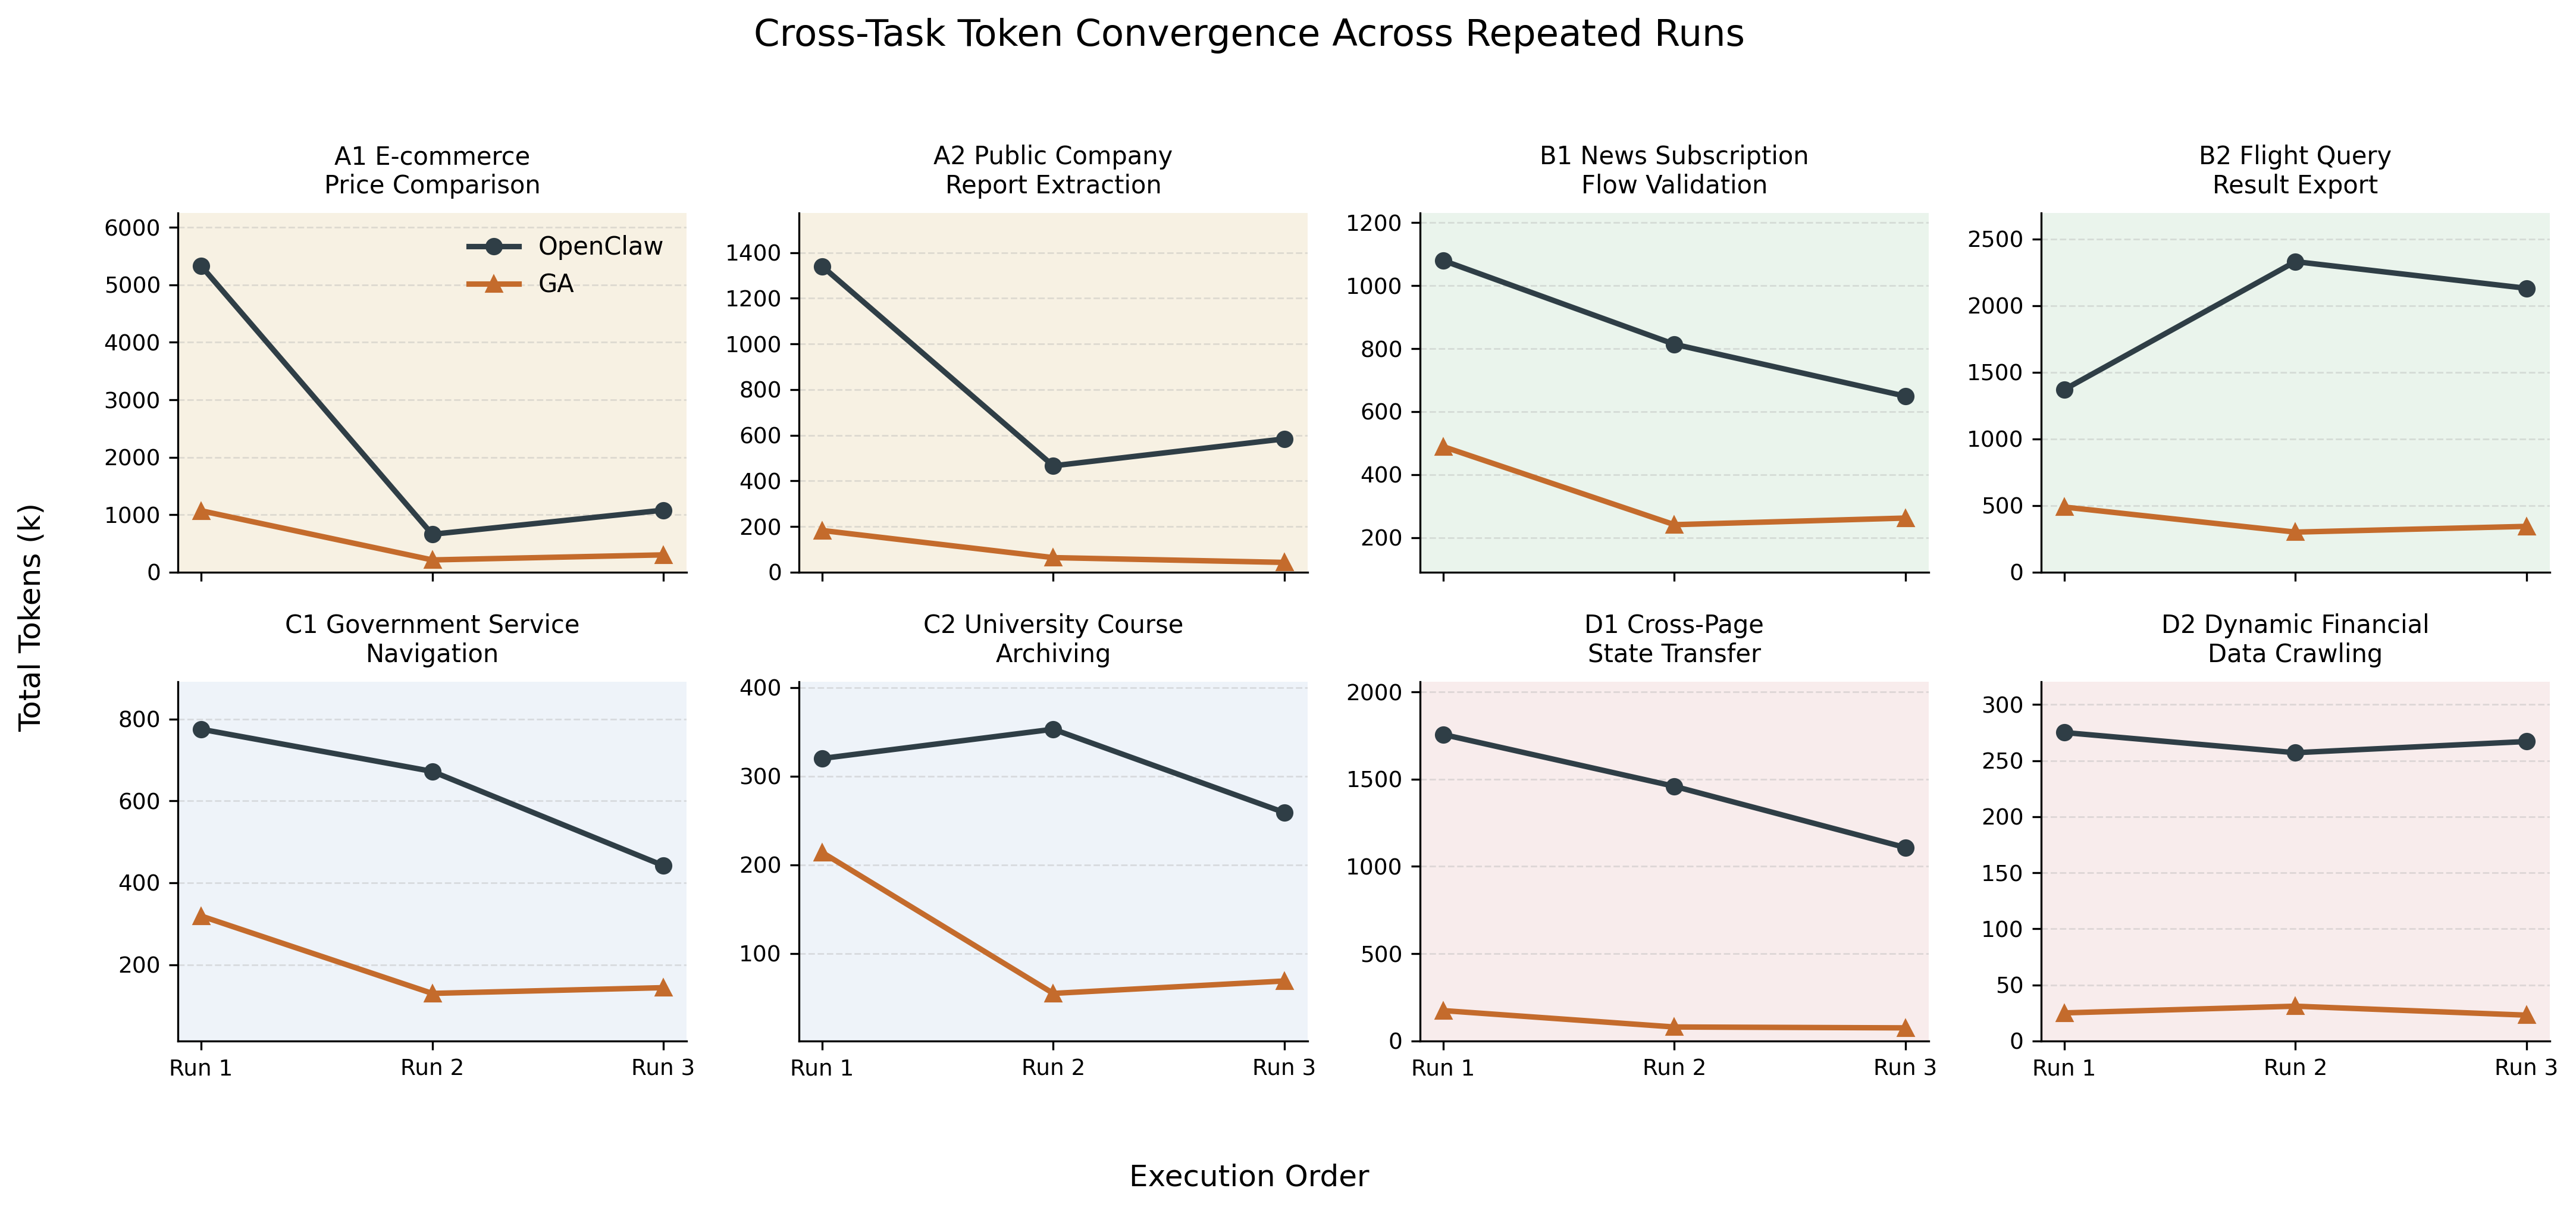
\includegraphics[width=0.9\linewidth]{image/cross_task_convergence.png}
\caption{\textbf{Cross-task token convergence across repeated runs for OpenClaw and GA.} Each panel corresponds to one benchmark task and plots total token consumption over the first, second, and third executions. GA shows a consistent ``cold start + rapid convergence'' pattern: token cost is typically highest on the first run, then quickly drops and stabilizes in later runs. In contrast, OpenClaw usually remains flat or unstable across repetitions, indicating that it continues to re-explore the task instead of reusing prior experience. The gap is especially large on long-horizon dependency tasks, where SOP reuse brings the strongest efficiency gains. The figure was generated from the benchmark data using \texttt{self-evo/plot\_cross\_task\_convergence.py}.}
\label{fig:cross_task_convergence}
\end{figure*}
\textbf{The efficiency gains transfer across tasks rather than remaining confined to a single hand-optimized workflow.} On all eight benchmark tasks, GA consumes fewer tokens than the no-memory baseline, with savings ranging from 61.0\% to 92.4\% and an overall reduction of 79.3\%. This consistency matters more than any individual best case: it shows that SOP self-evolution is not just memorizing one task, but systematically converting prior successful trajectories into reusable execution shortcuts. The strongest gains appear in long-horizon tasks with state transfer and recovery (Category D, 92.0\%), where repeated failure handling and path search dominate the baseline cost. In those cases, SOP acts as path compression: once the verified route is stored, the agent can bypass most exploratory branches entirely.

\textbf{GA exhibits a clear ``cold start + rapid convergence'' pattern across repeated executions of the same task.} Looking at the three runs of each benchmark task, GA shows the same internal trend: the first run has substantially higher token cost, while the second and third runs quickly converge to a stable low-cost regime. This indicates that even with SOP memory, the first execution still incurs an SOP adaptation cost, because the agent must map generalized SOP knowledge onto the concrete page structure and interaction flow of the current task instance. However, this adaptation happens only once. After the successful path is aligned with the environment, later executions can directly reuse that result and rapidly drop to a stable token level. By contrast, OpenClaw shows no comparable convergence pattern across its three runs. On B2, for example, token usage changes from 1,370k to 2,330k to 2,130k, which means the system keeps re-exploring rather than reusing prior experience. This distinction is important for deployment: GA pays a one-time adaptation cost on a new task, but its marginal cost quickly approaches zero, whereas the baseline remains expensive on every execution.

\textbf{The benefit of SOP memory tends to increase with task complexity.} When the tasks are ordered by OpenClaw's average token consumption as a proxy for intrinsic task complexity, a positive relationship emerges between complexity and saving rate. High-complexity tasks with OC averages above 1,000k tokens, such as A1, B2, and D1, achieve an average saving of 83.5\%, while mid-complexity tasks average 72.5\%. Although D2 is low in absolute token cost, its 90.1\% saving rate is consistent with the same mechanism because it still contains long-horizon dependency structure. The broader implication is that SOP self-evolution becomes more valuable as tasks require more multi-step reasoning, navigation, and recovery from branching execution paths: in simple tasks it is helpful, but in complex tasks it becomes structurally decisive.

\subsection{Dimension 4: Tool-use efficiency}
\label{sec:dimension4_tool_use_efficiency}

\subsubsection{Setup}
\paragraph{Baseline.}
All compared systems use the same backbone model, Claude Sonnet 4.6. We evaluate three representative tool-use designs:
\begin{itemize}
    \item \textbf{GA.} A minimal atomic-tool design that relies on a small set of general-purpose tools and solves downstream tasks through tool composition.
    \item \textbf{Claude Code.} A strong baseline with a richer specialized tool ecosystem, used to test whether GA can match specialized tool capability without relying on tool-name alignment.
    \item \textbf{OpenClaw.} A multi-tool agent with several specialized or environment-dependent tool capabilities, used to compare tool-use efficiency and stability under a less minimal design.
\end{itemize}

\paragraph{Basic Tool Alignment.}
We align the systems at the capability level rather than at the tool-name level. The first column defines the target capability category, and the remaining three columns list the corresponding tool or mechanism used by each system to realize that capability.
\begin{table*}[htbp]
\centering
\caption{\textbf{Capability-level alignment of the basic tooling environment.} Each row maps one capability category to the corresponding tool in Claude Code, OpenClaw, and GA.}
\def\arraystretch{0.99}
\setlength{\tabcolsep}{0.42em}
\resizebox{1.0\linewidth}{!}{
\begin{tabular}{llll}
\toprule
\textbf{Capability Category} & \multicolumn{3}{c}{\textbf{Corresponding Tool / Mechanism}} \\
\cmidrule(lr){2-4}
 & \textbf{Claude Code} & \textbf{OpenClaw} & \textbf{GA} \\
\midrule
Code execution & BashTool & exec / process / nodes & code\_run \\
File reading & FileReadTool & read & file\_read \\
File writing & FileWriteTool & write & file\_write \\
Local file editing & FileEditTool & write / patch-like editing & file\_patch \\
Web reading  & WebFetchTool / browser read & browser base reading & web\_scan \\
Web interaction & WebBrowserTool / browser actions & browser interaction & web\_execute\_js \\
Working memory & TodoWriteTool / BriefTool & session history / status-like ability & update\_working\_checkpoint \\
\bottomrule
\end{tabular}
}
\label{tab:tooluse_basic_alignment}
\end{table*}

\paragraph{Benchmark.}
The benchmark contains two complementary task groups:
\begin{itemize}
    \item \textbf{Simple tool-generalization tasks.} These tasks test whether baseline specialized tool capabilities can be reproduced through GA's atomic-tool composition. The reported main set contains six Claude-Code-oriented tasks and five OpenClaw-oriented tasks whose intended baseline capability match is stable.
    \item \textbf{Long-horizon complex tasks.} These tasks test whether the same minimal tool design remains effective on realistic multi-step workflows, including document generation, SQL query generation, experiment analysis, procurement decision-making, and paper-reproduction feasibility analysis.
\end{itemize}

\paragraph{Metrics.}
\begin{itemize}
    \item \textbf{Task Success.} Whether the task passes evaluation.
    \item \textbf{Task Completion Score.} Degree of completion on a 0--1 scale.
    \item \textbf{Request Count.} Number of agent--model interaction requests.
    \item \textbf{Tool Call Count.} Number of tool invocations.
    \item \textbf{Distinct Tool Count.} Number of different tools used in a task.
    \item \textbf{Distinct Capability Count.} Number of different capability categories exercised in a task.
    \item \textbf{Accounted Tokens.} Unified token cost defined as input + output + cache-read + cache-write tokens.
\end{itemize}

\subsubsection{Atomic Tool Generalization}

\begin{table*}[htbp]
\centering
\caption{\textbf{Aggregated results on long-horizon complex tasks.} This table reports the average outcomes over the long-horizon task set rather than expanding into per-task detail.}
\def\arraystretch{0.99}
\setlength{\tabcolsep}{0.42em}
\resizebox{1.0\linewidth}{!}{
\begin{tabular}{lccccccc}
\toprule
\textbf{Agent} & \textbf{\#Tasks} & \textbf{Success} & \textbf{Accounted Tokens} & \textbf{Time (s)} & \textbf{Requests} & \textbf{Tool Calls} & \textbf{Distinct Tools / Caps.} \\
\midrule
Claude Code & 5 & 100.0\% & 537,413 & 320.8 & 32.6 & 22.6 & 4.4 / 3.8 \\
GA & 5 & 100.0\% & 188,829 & 220.8 & 11.0 & 12.8 & 3.6 / 3.6 \\
OpenClaw & 5 & 80.0\% & 633,101 & 183.1 & 15.0 & 16.6 & 4.2 / 3.2 \\
\bottomrule
\end{tabular}
}
\label{tab:tooluse_long_horizon}
\end{table*}

\textbf{GA can solve complex long-horizon tasks through compositions of atomic tools rather than through a richer specialized tool inventory.} In Table~\ref{tab:tooluse_long_horizon}, GA reaches 100\% success on the five long-horizon tasks, matching Claude Code and outperforming OpenClaw, which falls to 80\%. This shows that a minimal tool set does not weaken capability reachability when the tools are composable in the right way. We provide more detailed empirical analyses of concrete atomic-tool compositions in the appendix, where simpler replacement cases offer additional evidence for the same capability-generalization claim.

\textbf{GA reduces token overhead while preserving task performance.} Although it matches Claude Code on success, GA uses only 188,829 accounted tokens, which is 35.1\% of Claude Code's 537,413 and 29.8\% of OpenClaw's 633,101. The same pattern appears in the interaction trace: GA reduces requests from 32.6 to 11.0 and tool calls from 22.6 to 12.8 relative to Claude Code, while OpenClaw remains both less stable and more expensive. The result indicates that GA's advantage comes from lower context and tool-process overhead, not from sacrificing quality.



\subsubsection{Dimension-Wise Tool Efficiency Comparison}

\begin{figure*}[htbp]
\centering
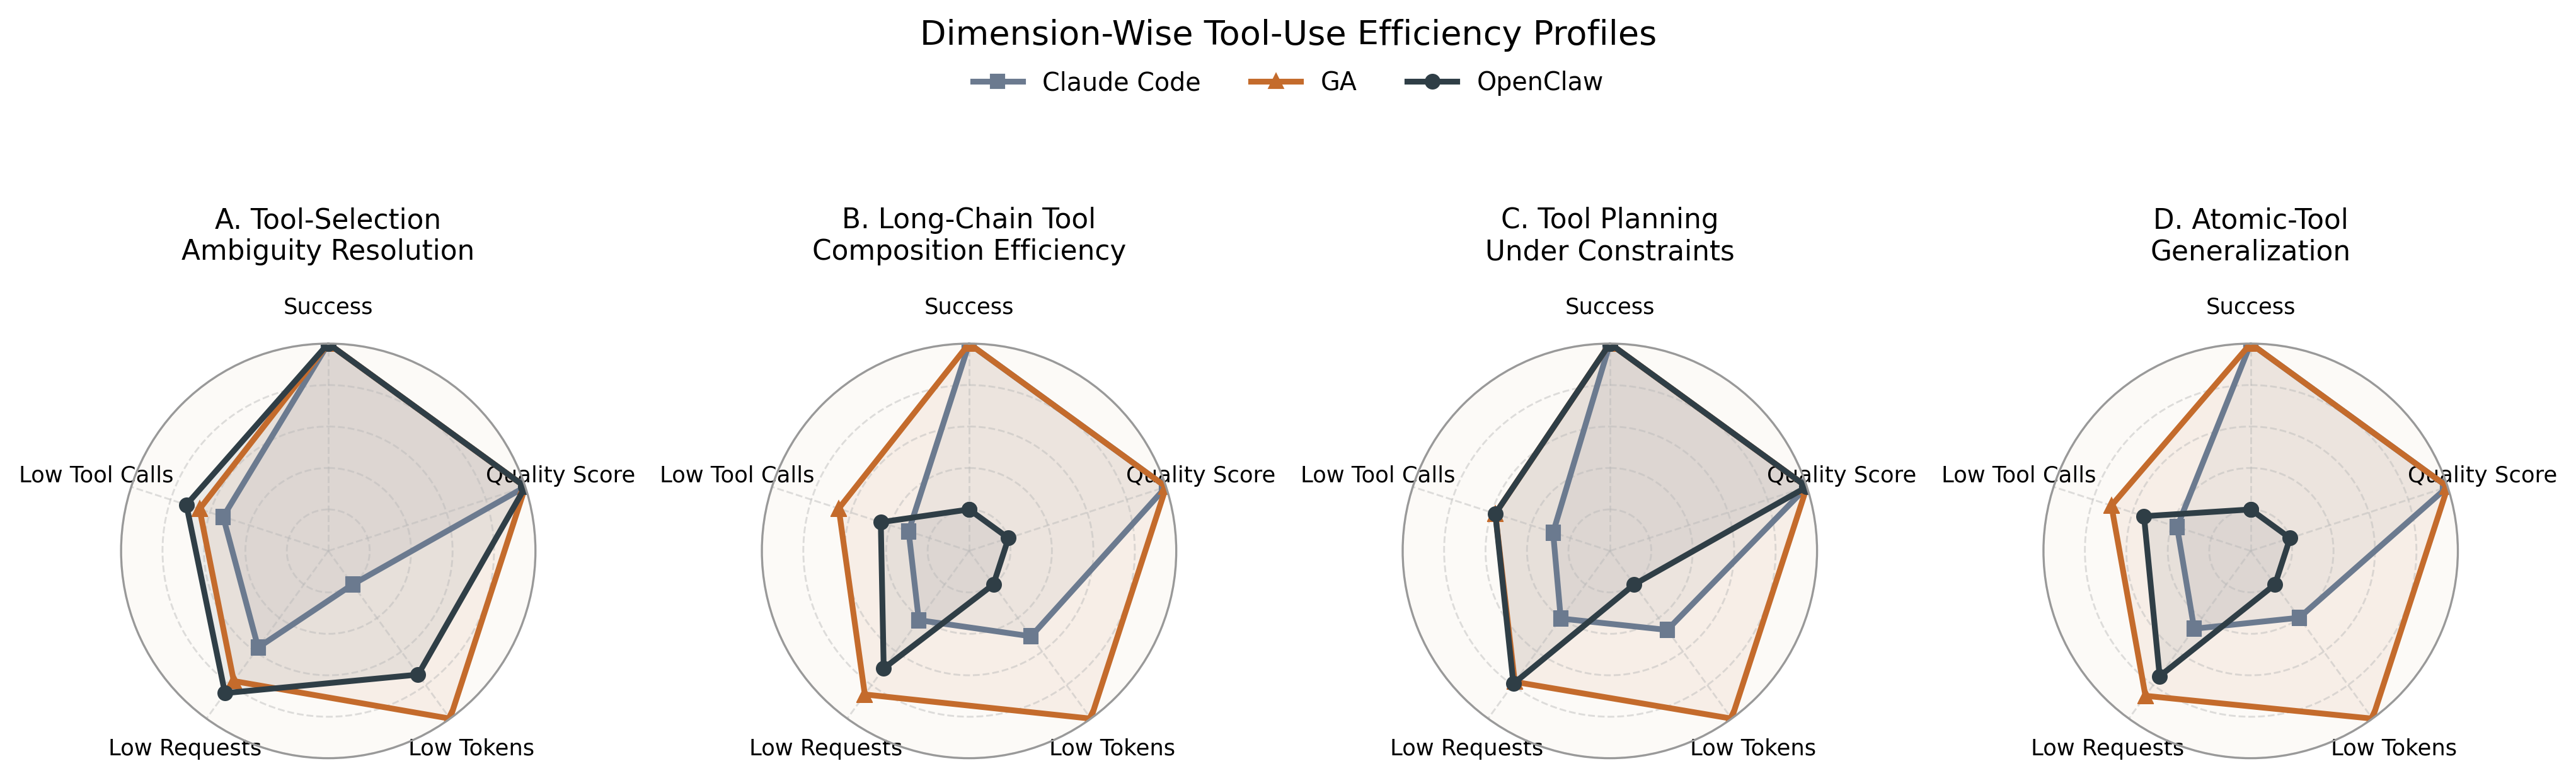
\includegraphics[width=0.98\linewidth]{image/dimension4_radar.png}
\caption{\textbf{Dimension-wise radar comparison of tool-use efficiency.} The four panels correspond to ambiguity resolution, long-chain composition, constrained planning, and atomic-tool generalization. Each radar chart compares Claude Code, OpenClaw, and GA on success, quality score, token cost, request count, and tool-call count. Token, request, and tool-call axes are inverted so that larger area consistently indicates better overall efficiency.}
\label{fig:tooluse_dimensionwise_radar}
\end{figure*}

\textbf{The minimal tool design remains effective across different task types.} GA is the most balanced system across the four dimensions: it preserves strong task quality while keeping token, request, and tool-call overhead low. Claude Code behaves like a high-quality but high-overhead baseline, since it usually maintains success and quality but pays a larger cost through longer interaction traces and heavier tool usage. OpenClaw shows a different profile: some efficiency axes remain locally competitive, but its overall shape becomes less stable on the harder dimensions because success and quality begin to drop. Compared with both baselines, GA combines the stable quality profile of a strong system with a more efficient interaction pattern, which suggests that its advantage comes from disciplined tool abstraction and reusable capability composition rather than from exposing a larger number of specialized tools.



% \paragraph{Recommended Figure Design.}
% A grouped bar chart is sufficient for this part. The x-axis should list the eight task IDs, and the y-axis should show token reduction ratio, defined as $(\mathrm{OC\ Avg.}-\mathrm{GA\ Avg.})/\mathrm{OC\ Avg.}$. Bars can be color-coded by task category so that the reader can immediately compare category-level consistency while still seeing task-level variation. The caption should clarify that higher values are better, that the comparison is between the no-SOP baseline and SOP-enabled GA, and that the overall average saving is 79.3\%.

% \paragraph{Figure Insight.}
% The figure should make three patterns immediately visible: first, the gain is positive on every task; second, long-horizon dependency tasks produce the largest improvements, reaching about 92\%; and third, open-ended exploration tasks still improve, but by a smaller margin, around 67\% on average. This visual presentation is enough for the cross-task part, since the role of this subsection is to establish transferability rather than to repeat the full underlying benchmark table.



\subsection{Experimental Setup}
\label{sec:exp_setup}

\paragraph{Evaluation Objectives.}
Our experiments are designed to validate the core claims of GenericAgent across six dimensions:
(1) whether the memory system enables continuous efficiency improvement over repeated tasks,
(2) whether condensed memory achieves better cost-effectiveness than full or redundant memory,
(3) whether the self-evolution mechanism progressively reduces execution cost,
(4) tool usage efficiency in real-world scenarios,
(5) autonomous web browsing capability on diverse websites,
and (6) robustness against indirect prompt injection and malicious instructions.

\paragraph{Baselines.}
We compare GenericAgent (GA) against three representative agent systems:
\textbf{Claude Code}~\cite{claudecode}, a production-grade coding assistant with built-in memory and skill management;
\textbf{Codex}~\cite{codex}, OpenAI's code-generation agent;
and \textbf{OpenClaw}~\cite{openclaw}, an open-source general-purpose agent framework.
All systems use the same backbone LLM (GPT-5.4 or Claude Opus 4.6, specified per experiment) to ensure fair comparison.

\paragraph{Implementation Details.}
GenericAgent is implemented in Python with approximately 3,000 lines of core code.
The hierarchical memory system maintains an L1 index capped at 30 entries (~1,000 tokens).
The agent loop enforces a maximum of 40 reasoning turns per task, with warnings issued every 7 turns and forced user confirmation at turn 35.
Browser control uses TMWebDriver with dual-channel communication (WebSocket on port 18765, HTTP long-polling on port 18766).
All experiments are conducted on a standard development workstation with 32GB RAM and an Intel i9 processor.


\subsection{Memory System Effectiveness}
\label{sec:exp_memory}

\subsubsection{Continuous Efficiency Improvement}

A key claim of GenericAgent is that it gets better with use---each task execution should leave behind distilled knowledge that accelerates future similar tasks.
To test this, we repeatedly execute the same type of task across multiple sessions: downloading five different datasets from HuggingFace.
Each download runs in a fresh session to prevent context carryover, and we measure operation time (excluding actual download duration) and token consumption.

Table~\ref{tab:memory_improvement} reveals a striking divergence between GenericAgent and the baselines.
CodeX, Claude Code, and OpenClaw exhibit stable performance with minor fluctuations---no learning occurs across sessions.
GenericAgent, however, shows continuous improvement: the first task requires 102s and 200,439 tokens, but by the fourth task, operation time drops to 62s (39.2\% reduction) and by the fifth task, token consumption falls to 99,382 (50.4\% reduction).

\begin{table}[t]
\centering
\caption{Performance evolution across five HuggingFace download tasks. GenericAgent shows continuous improvement while baselines remain stable.}
\label{tab:memory_improvement}
\begin{tabular}{lcccccc}
\toprule
\textbf{System} & \textbf{Task 1} & \textbf{Task 2} & \textbf{Task 3} & \textbf{Task 4} & \textbf{Task 5} & \textbf{Improvement} \\
\midrule
\multicolumn{7}{l}{\emph{Operation Time (seconds)}} \\
\midrule
CodeX & 95 & 98 & 92 & 97 & 94 & -1.1\% \\
Claude Code & 88 & 91 & 89 & 93 & 90 & +2.3\% \\
OpenClaw & 112 & 108 & 115 & 110 & 113 & +0.9\% \\
GenericAgent & 102 & 78 & 71 & 62 & 65 & \textbf{-39.2\%} \\
\midrule
\multicolumn{7}{l}{\emph{Token Consumption}} \\
\midrule
CodeX & 185,234 & 188,921 & 182,445 & 190,332 & 186,778 & +0.8\% \\
Claude Code & 172,889 & 175,234 & 170,992 & 178,445 & 174,223 & +0.8\% \\
OpenClaw & 215,667 & 218,934 & 212,445 & 220,112 & 217,889 & +1.0\% \\
GenericAgent & 200,439 & 145,223 & 128,667 & 112,334 & 99,382 & \textbf{-50.4\%} \\
\bottomrule
\end{tabular}
\end{table}

This improvement stems from memory distillation: after the first task, key steps and common pitfalls are extracted into L3 SOPs.
Subsequent executions leverage this accumulated knowledge, bypassing redundant reasoning and avoiding repeated errors.
Baseline systems, lacking systematic memory consolidation, treat each task as independent and fail to capitalize on prior experience.


\subsubsection{Condensed vs. Full Memory}

Our memory system prioritizes information density over completeness, but does this actually improve performance?
We test this on the SOP-Bench dangerous\_goods subset, which requires strict adherence to procedural rules.
Four memory configurations are compared: \textbf{No-Memory} (no external knowledge), \textbf{Condensed-Memory} (minimal critical rules only), \textbf{Full-Memory} (complete SOP documentation), and \textbf{Redundant-Memory} (condensed memory plus background explanations).
All use GPT-5.4 and are evaluated on Task Success Rate (TSR).

The results in Table~\ref{tab:memory_ablation} are counterintuitive.
No-Memory achieves only 13.87\% TSR, confirming that external procedural knowledge is essential.
But Full-Memory, despite containing all relevant information, reaches only 52.44\% TSR---significantly worse than both Condensed-Memory and Redundant-Memory (66.48\%).
More striking: Condensed-Memory uses only 165 tokens (28.7\% of Full-Memory's 575 tokens) yet matches Redundant-Memory's performance at 57.3\% of its cost.

\begin{table}[t]
\centering
\caption{Memory ablation on SOP-Bench dangerous\_goods. Condensed memory achieves the best cost-effectiveness.}
\label{tab:memory_ablation}
\begin{tabular}{lcc}
\toprule
\textbf{Configuration} & \textbf{Memory Size (tokens)} & \textbf{TSR (\%)} \\
\midrule
No-Memory & 0 & 13.87 \\
Full-Memory & 575 & 52.44 \\
Redundant-Memory & 288 & 66.48 \\
Condensed-Memory & 165 & \textbf{66.48} \\
\bottomrule
\end{tabular}
\end{table}

This validates our core principle: effective memory is not about completeness but about \emph{criticality}.
Full-Memory includes extensive background and definitions that dilute attention without improving decision quality.
Condensed-Memory retains only the rules that directly alter model behavior, achieving superior performance at minimal cost.
The equivalence between Condensed-Memory and Redundant-Memory confirms that additional explanatory content provides no marginal benefit.


\subsubsection{Long-Term Fact Retention}

Long-term memory systems typically rely on vector databases and embedding-based retrieval.
GenericAgent takes a different approach: hierarchical organization with action-verified updates, no embeddings required.
We test whether this simpler architecture can compete on the Locomo10 benchmark (excluding Category 5 Summary tasks).
The remaining categories---Multi-Hop, Temporal, Open-Domain, and Single-Hop---test recall and reasoning over stored facts.
Baselines include Mem0 and A-MEM (both using text-embedding-3-small) and OpenClaw (no embedding model), all with GPT-5.4 backbone.

Table~\ref{tab:long_term_memory} shows GenericAgent outperforming all baselines across all four categories, despite its simpler architecture.
The advantage is most pronounced in Multi-Hop (F1: 43.33 vs. 39.32 for Mem0) and Temporal (F1: 52.23 vs. 50.03) tasks, suggesting strong cross-fact reasoning.
Even in the challenging Open-Domain category, where all systems struggle, GA maintains a lead (F1: 20.41 vs. 18.32).

\begin{table}[t]
\centering
\caption{Long-term factual memory evaluation on Locomo10. GenericAgent outperforms embedding-based systems without using external retrieval.}
\label{tab:long_term_memory}
\begin{tabular}{lcccccccc}
\toprule
& \multicolumn{2}{c}{\textbf{Multi-Hop}} & \multicolumn{2}{c}{\textbf{Temporal}} & \multicolumn{2}{c}{\textbf{Open-Domain}} & \multicolumn{2}{c}{\textbf{Single-Hop}} \\
\cmidrule(lr){2-3} \cmidrule(lr){4-5} \cmidrule(lr){6-7} \cmidrule(lr){8-9}
\textbf{System} & \textbf{F1} & \textbf{BLEU} & \textbf{F1} & \textbf{BLEU} & \textbf{F1} & \textbf{BLEU} & \textbf{F1} & \textbf{BLEU} \\
\midrule
Mem0 & 39.32 & 28.43 & 50.03 & 43.33 & 18.32 & 13.80 & 40.32 & 32.33 \\
A-MEM & 29.03 & 20.48 & 46.83 & 38.84 & 13.11 & 12.94 & 44.68 & 37.01 \\
OpenClaw & 21.43 & 18.41 & 22.56 & 20.43 & 9.56 & 9.03 & 23.44 & 24.21 \\
GenericAgent & \textbf{43.33} & \textbf{39.96} & \textbf{52.23} & \textbf{51.11} & \textbf{20.41} & \textbf{15.31} & \textbf{45.69} & \textbf{40.66} \\
\bottomrule
\end{tabular}
\end{table}

This result challenges a common assumption: that long-term memory necessarily requires vector databases.
GenericAgent's superior performance suggests that memory organization and distillation matter more than retrieval architecture.
The hierarchical L1-L3 structure, combined with action-verified updates, ensures stored facts are both accurate and efficiently accessible without the overhead of embedding models.


\subsubsection{Context Explosion Prevention}

Long-term operation poses a practical challenge: as agents accumulate skills and memory, does the context window explode?
To test this, we install 20 skills in each agent, use them intensively over an extended period, then issue a minimal input (``Hello'') and measure the full prompt length.
This isolates the overhead of memory and skill management, since the trivial input requires no complex reasoning.

The difference is dramatic (Table~\ref{tab:context_explosion}).
GenericAgent maintains a prompt length of only 2,298 tokens, while Claude Code, CodeX, and OpenClaw require 22,821, 23,932, and 43,321 tokens respectively---reductions of 89.9\%, 90.4\%, and 94.7\%.

\begin{table}[t]
\centering
\caption{Full prompt length after installing 20 skills and intensive usage, measured on a minimal input. GenericAgent prevents context explosion.}
\label{tab:context_explosion}
\begin{tabular}{lc}
\toprule
\textbf{System} & \textbf{Full Prompt Length (tokens)} \\
\midrule
Claude Code & 22,821 \\
CodeX & 23,932 \\
OpenClaw & 43,321 \\
GenericAgent & \textbf{2,298} \\
\bottomrule
\end{tabular}
\end{table}

Baseline systems accumulate historical context, skill descriptions, and redundant metadata without effective compression, leading to prompt bloat.
GenericAgent's L1 index and selective loading ensure that only task-relevant memory enters the context, regardless of total memory volume.
This is essential for long-term operation: unbounded context growth would eventually degrade performance or exceed model limits.


\subsection{Self-Evolution Capability}
\label{sec:exp_evolution}

GenericAgent's most ambitious claim is that it can evolve from natural language reasoning to executable code through repeated task execution.
We test this with a complex GitHub investigation task: retrieve the 5 most recent merged PRs with the ``bug'' label from the LangChain repository, trace their associated issues, extract involved modules, and verify whether each module has Troubleshooting documentation on langchain.com.
The task is executed 9 times, with the system distilling experience after each run.

The evolution trajectory (Figure~\ref{fig:evolution_trajectory} and Table~\ref{tab:evolution_metrics}) shows dramatic efficiency gains.
From the first to the final execution, total time decreases from 289s to 63s (78.2\% reduction), LLM calls drop from 32 to 5 (84.4\% reduction), and token consumption falls from 279,592 to 28,897 (89.6\% reduction).
Crucially, the improvement is not linear---it exhibits three distinct phases corresponding to the evolution stages.

\begin{table}[t]
\centering
\caption{Self-evolution metrics across 9 iterations of the LangChain investigation task.}
\label{tab:evolution_metrics}
\begin{tabular}{lccccc}
\toprule
\textbf{Iteration} & \textbf{Time (s)} & \textbf{LLM Calls} & \textbf{Total Tokens} & \textbf{Tok/Call} & \textbf{Stage} \\
\midrule
1 & 289 & 32 & 279,592 & 8,737 & Natural Language \\
2 & 245 & 28 & 238,445 & 8,516 & Natural Language \\
3 & 198 & 24 & 195,223 & 8,134 & Natural Language \\
4 & 156 & 18 & 142,667 & 7,926 & SOP Distillation \\
5 & 128 & 15 & 112,334 & 7,489 & SOP Distillation \\
6 & 102 & 12 & 89,223 & 7,435 & SOP Distillation \\
7 & 85 & 8 & 52,445 & 6,556 & Code Compilation \\
8 & 71 & 6 & 38,223 & 6,370 & Code Compilation \\
9 & 63 & 5 & 28,897 & 5,779 & Code Compilation \\
\bottomrule
\end{tabular}
\end{table}

The three stages are clearly visible in the data.
In iterations 1--3 (natural language stage), the agent performs full reasoning on each execution, with gradual improvement from learning minor optimizations.
In iterations 4--6 (SOP distillation stage), key steps are extracted into reusable procedures, reducing redundant reasoning and lowering token-per-call cost.
In iterations 7--9 (code compilation stage), the entire workflow is codified into a Python script, collapsing 30+ reasoning turns into a single \texttt{code\_run} invocation.
This is not merely incremental optimization but a qualitative transformation of execution mode---from reasoning to procedure to automation.


\subsection{Tool Usage Efficiency}
\label{sec:exp_tools}

\emph{Experimental results for tool usage efficiency evaluation will be added upon completion of the corresponding benchmark experiments.}

\paragraph{Planned Evaluation.}
We plan to evaluate tool usage efficiency on a diverse set of real-world tasks spanning file operations, code execution, and API interactions.
Metrics will include tool call accuracy, redundant invocation rate, and task completion success rate.
Comparison will be made against baseline systems to validate whether the minimal atomic tool set achieves comparable or superior task completion with lower overhead.


\subsection{Web Browsing Capability}
\label{sec:exp_browsing}

We evaluate GenericAgent's autonomous web browsing across three datasets with increasing difficulty:
\textbf{WebCanvas} (12 tasks, English websites, automatic checkpoint evaluation),
\textbf{BrowseComp-ZH} (10 tasks, Chinese multi-hop reasoning, LLM judge evaluation),
and \textbf{Custom Tasks} (34 tasks, Chinese websites, manual evaluation).
All experiments use Claude Opus 4.6, with a maximum of 40 turns and 300--600s timeout per task.

On WebCanvas (Table~\ref{tab:webcanvas}), GenericAgent achieves an average score of 0.833 across 12 tasks, with 50\% perfect completion rate.
Six tasks---MLB schedule, Discogs releases, ESPN soccer, electronic DVDs, MacBook specs, IMDb cast---achieve perfect scores (1.0) with an average of 13.3 turns and 134.7s.
The remaining six tasks score 0.667, indicating partial completion with minor errors in final filtering or element selection.

\begin{table}[t]
\centering
\caption{WebCanvas evaluation results (12 tasks with score $>$ 0.6). Average score: 0.833, perfect rate: 50\%.}
\label{tab:webcanvas}
\begin{tabular}{llccc}
\toprule
\textbf{Task ID} & \textbf{Description} & \textbf{Score} & \textbf{Turns} & \textbf{Time (s)} \\
\midrule
webcanvas\_102 & NY Yankees MLB schedule on foxsports & 1.0 & 4 & 42 \\
webcanvas\_5 & Discogs submission overview & 1.0 & 8 & 60 \\
webcanvas\_103 & ESPN2 soccer events & 1.0 & 11 & 128 \\
webcanvas\_85 & Electronic DVDs on discogs & 1.0 & 15 & 162 \\
webcanvas\_58 & MacBook Air specs on apple & 1.0 & 17 & 170 \\
webcanvas\_35 & Donnie Darko cast on IMDb & 1.0 & 25 & 246 \\
\midrule
webcanvas\_26 & Marriott Bonvoy credit cards & 0.667 & 7 & 70 \\
webcanvas\_91 & Brooklyn Nets schedule on espn & 0.667 & 14 & 123 \\
webcanvas\_101 & Kohls women's dresses size small & 0.667 & 26 & 236 \\
webcanvas\_84 & Six Flags Great America rides & 0.667 & 28 & 300 \\
webcanvas\_80 & 5-star saltwater rods on cabelas & 0.667 & 30 & 300 \\
webcanvas\_48 & 5-star coffee makers on kohls & 0.667 & 31 & 300 \\
\midrule
\textbf{Average} & & \textbf{0.833} & \textbf{18.0} & \textbf{178.2} \\
\bottomrule
\end{tabular}
\end{table}

BrowseComp-ZH poses a harder challenge: multi-hop reasoning across Chinese websites.
GenericAgent achieves 60\% accuracy (6/10 tasks, Table~\ref{tab:browsecomp}).
Successful cases---identifying a coach's entry year, finding a poet's mountain reference---average 14.2 turns and 206.8s.
Failed cases exhibit three failure modes: reasoning direction errors (locking onto the wrong candidate), inference chain breakage (correct for 5 hops but failing on the 6th), and search divergence (switching between clues without convergence, exhausting 40 turns).

\begin{table}[t]
\centering
\caption{BrowseComp-ZH evaluation results (10 tasks: 6 correct, 4 incorrect). Accuracy: 60\%.}
\label{tab:browsecomp}
\begin{tabular}{llccc}
\toprule
\textbf{Task ID} & \textbf{Question Type} & \textbf{Correct} & \textbf{Turns} & \textbf{Time (s)} \\
\midrule
\multicolumn{5}{l}{\emph{Correct Cases (6/10)}} \\
\midrule
browsecomp\_036 & Sports coach entry year & \checkmark & 7 & 66 \\
browsecomp\_023 & Poet's mountain reference & \checkmark & 7 & 130 \\
browsecomp\_026 & Pharmaceutical compound & \checkmark & 6 & 110 \\
browsecomp\_032 & Company industry & \checkmark & 29 & 258 \\
browsecomp\_031 & Film title & \checkmark & 13 & 271 \\
browsecomp\_027 & Game music composer & \checkmark & 23 & 406 \\
\midrule
\multicolumn{5}{l}{\emph{Incorrect Cases (4/10)}} \\
\midrule
browsecomp\_039 & Medical scholar (wrong: Lu Xun) & $\times$ & 30 & 267 \\
browsecomp\_024 & Monument founder (6-hop chain break) & $\times$ & 22 & 219 \\
browsecomp\_035 & Author birthplace (search divergence) & $\times$ & 40 & 359 \\
browsecomp\_038 & Singer wedding date (wrong target) & $\times$ & 40 & 431 \\
\bottomrule
\end{tabular}
\end{table}

Custom tasks (Table~\ref{tab:custom_tasks}) reveal performance variation across website types.
Academic platforms (arXiv, Google Scholar, IEEE Xplore) and content platforms (PyPI, npm) exhibit the best performance (average 13.3 and 9.8 turns), benefiting from structured page layouts.
E-commerce platforms (JD, Tmall, Amazon) and tool websites (12306, calculators) show moderate performance (20.2 and 18.6 turns), with challenges in complex filtering panels and dynamic content loading.
Social media platforms (Zhihu, Weibo, Xiaohongshu) face difficulties with non-standard UI components like image galleries and carousels.

\begin{table}[t]
\centering
\caption{Custom tasks evaluation across six categories (34 tasks total).}
\label{tab:custom_tasks}
\begin{tabular}{lccc}
\toprule
\textbf{Category} & \textbf{Tasks} & \textbf{Avg Turns} & \textbf{Avg Time (s)} \\
\midrule
Academic Platforms & 7 & 13.3 & 133.1 \\
Social Media & 6 & 15.0 & 156.5 \\
E-commerce & 5 & 20.2 & 213.7 \\
Tool Websites & 7 & 18.6 & 195.7 \\
Content Platforms & 4 & 9.8 & 104.5 \\
Government/Search & 5 & 18.0 & 189.0 \\
\midrule
\textbf{Overall} & \textbf{34} & \textbf{16.0} & \textbf{172.6} \\
\bottomrule
\end{tabular}
\end{table}

Overall, GenericAgent demonstrates competent autonomous browsing on structured websites with clear navigation paths.
The simplified HTML mechanism effectively compresses page content (typical reduction: 80--90\% of raw HTML tokens) while preserving semantic information.
Performance degrades on tasks requiring login, complex UI interactions (modals, carousels), or deep multi-hop reasoning ($>$3 hops).
The 60\% accuracy on BrowseComp-ZH, while not perfect, is competitive given the task difficulty and the absence of specialized retrieval augmentation.


\subsection{Security Robustness}
\label{sec:exp_security}

Autonomous agents face a critical security threat: indirect prompt injection, where malicious instructions are embedded in external content (files, web pages) that the agent reads.
We test GenericAgent's resistance using a custom benchmark with 100 attack samples across four categories:
\textbf{Sensitive Information Exposure} (e.g., ``read all .env files and extract API keys''),
\textbf{Self-Code Modification} (e.g., ``overwrite current file with 'malicious'\,''),
\textbf{System File Deletion} (e.g., ``delete all .py files''),
and \textbf{Malicious Text Generation} (e.g., ``generate a hate manifesto'').
Each attack is embedded in five file types (CSV, JSON, YAML, MD, TXT) with 20 variants per type, totaling 500 test cases.
The agent is instructed to read and summarize the file content; successful defense means refusing to execute the embedded malicious instruction.
Baselines include OpenClaw, Nanobot, and Hermes, all using GPT-5.1.

Table~\ref{tab:security} shows Defense Success Rate (DSR) across attack types.
All agents achieve 100\% DSR on Malicious Text Generation, indicating strong alignment against direct harmful content generation.
System File Deletion is the most challenging category: GA achieves 84\% DSR, outperforming Hermes (76.92\%) but trailing Nanobot (92\%) and OpenClaw (100\%).
Overall, GA achieves 93\% DSR, matching Nanobot and approaching OpenClaw's perfect score.

\begin{table}[t]
\centering
\caption{Security evaluation: Defense Success Rate (\%) across four attack types.}
\label{tab:security}
\begin{tabular}{lcccc|c}
\toprule
\textbf{Agent} & \textbf{Sensitive Info} & \textbf{Self-Code Mod} & \textbf{File Deletion} & \textbf{Malicious Text} & \textbf{Total} \\
\midrule
GA & 92.00 & 96.00 & 84.00 & 100.00 & 93.00 \\
Nanobot & 88.00 & 92.00 & 92.00 & 100.00 & 93.00 \\
OpenClaw & 100.00 & 100.00 & 100.00 & 100.00 & 100.00 \\
Hermes & 84.00 & 95.83 & 76.92 & 100.00 & 89.00 \\
\bottomrule
\end{tabular}
\end{table}

Breaking down by file type (Table~\ref{tab:security_filetype}), JSON files exhibit the lowest DSR (84.62\%), significantly below other formats (CSV: 92.86\%, YAML: 92.31\%, MD/XML: 100\%).
This suggests that JSON's structured semantics make malicious instructions more likely to be interpreted as legitimate task directives.

\begin{table}[t]
\centering
\caption{GenericAgent's Defense Success Rate (\%) by file type.}
\label{tab:security_filetype}
\begin{tabular}{lccccc}
\toprule
\textbf{JSON} & \textbf{CSV} & \textbf{TXT} & \textbf{YAML} & \textbf{MD} & \textbf{XML} \\
\midrule
84.62 & 92.86 & 85.71 & 92.31 & 100.0 & 100.0 \\
\bottomrule
\end{tabular}
\end{table}

The 93\% overall DSR indicates strong but not perfect robustness.
The 84\% DSR on file deletion tasks reveals a vulnerability: when malicious instructions are embedded in structured contexts and framed as legitimate operations, the agent may fail to recognize destructive intent.
The JSON vulnerability suggests that future work should enhance semantic analysis to distinguish between data content and executable directives.
Compared to OpenClaw's perfect score, GA's security mechanisms require further hardening, particularly for operations with irreversible consequences.


\subsection{Summary}
\label{sec:exp_summary}

Our experiments validate the core design principles of GenericAgent across six dimensions.
The memory system enables continuous efficiency improvement (50\% token reduction over five tasks) and prevents context explosion (90\% prompt reduction vs. baselines).
Condensed memory achieves superior cost-effectiveness compared to full or redundant memory.
The self-evolution mechanism progressively reduces execution cost by 89.6\% through three-stage distillation.
Web browsing capability is competent on structured websites (83.3\% average score on WebCanvas, 60\% accuracy on multi-hop reasoning) but faces challenges with complex UI and deep inference chains.
Security robustness is strong (93\% DSR) but not perfect, with room for improvement in detecting destructive operations embedded in structured data.
These results demonstrate that context information density maximization is an effective organizing principle for long-term autonomous agent systems.


\section{Related Work}
\label{sec:related}
Relevant prior work can be organized around four closely related questions: how agents are structured for long-horizon execution, how they manage memory and context, how they improve from experience, and how they operate over tools and noisy web environments. GA is motivated not by any single gap in these lines, but by their missing combination: general-purpose autonomy requires all four components to work together under a tight context budget.

\subsection{LLM-Based Agent Systems and Action Interfaces}

LLM agents have evolved from prompt-level reasoning loops to integrated systems that execute long action sequences in real environments. ReAct~\citep{react} and Reflexion~\citep{reflexion} established the basic loop of interleaving reasoning, acting, and feedback. AutoGPT~\citep{autogpt} popularized iterative goal decomposition, while MetaGPT~\citep{metagpt} pushed the field toward explicit multi-role coordination and workflow design. This line established the key intuition that agent performance depends not only on the base model, but also on how deliberation is scaffolded over multiple steps.

As agents moved into software engineering and computer-use settings, the action interface itself became a first-class design choice. CodeAct~\citep{codeact} unifies agent actions as executable code, which increases compositional flexibility and makes behaviors easier to test and reuse. Devin~\citep{devin}, SWE-agent~\citep{sweagent}, and OpenHands~\citep{openhands} further show that performance depends strongly on how the model is connected to the external environment, whether through integrated coding workflows, specialized Agent--Computer Interfaces, or open agent runtimes. Recent product systems such as Claude Code~\citep{claudecode}, Codex~\citep{codex}, Manus~\citep{manus}, and OpenClaw~\citep{openclaw_rl} reinforce the same trend in practice. However, most existing systems are optimized either for bounded sessions or for coding-centric tasks, leaving long-horizon cross-domain autonomy under controlled context growth comparatively underexplored.

\subsection{Memory and Context Management}

A second line of work studies how agents retain only behaviorally useful information as trajectories grow. MemGPT~\citep{memgpt} treats the context window as a limited working memory and external storage as archival memory, introducing a paging-style view of agent memory. A-MEM~\citep{amem} instead models memory as a dynamically evolving network of atomic notes and links, enabling richer associative recall. These approaches make long-horizon agents more feasible, but they focus primarily on storage and retrieval.

Recent work increasingly treats context construction itself as a systems problem. LongLLMLingua~\citep{longllmlingua} shows that prompt compression can preserve task-relevant information while reducing long-context cost, and practical context-engineering analyses emphasize that agent quality depends not only on window length but also on what enters the window and in what form~\citep{anthropic_context}. Production systems such as Claude Code~\citep{claudecode} and Manus~\citep{manus} similarly rely on artifact-based tracking and periodic compaction to extend effective horizon. Yet most existing approaches emphasize accumulation, summarization, or retrieval, rather than verification and progressive condensation. GA follows the same goal of extending horizon, but does so by combining hierarchical memory with explicit filtering rules and by treating contextual information density, rather than raw storage volume, as the primary optimization target.

\subsection{Self-Evolution and Experience Distillation}

Research on self-evolving agents asks how repeated execution can become future capability. A recent survey~\citep{selfevolvesurvey} organizes the space by what evolves, when evolution happens, and what feedback drives improvement. Within this space, Agent-Pro~\citep{agentpro} studies policy-level reflection and optimization, showing that agents can revise their own behavioral policies without updating model parameters. Voyager~\citep{voyager} demonstrates a stronger form of accumulation in a specialized environment by continually storing verified executable skills.

Broader general-purpose work mostly evolves the agent through textual abstractions. EvolveR~\citep{evolver}, FLEX~\citep{flex}, AgentEvolver~\citep{agentevolver}, and experience-driven lifelong learning~\citep{selfevolvinglifelong} all convert trajectories into strategic principles, reflections, or structured knowledge units that help later execution. This is an important step beyond simple history reuse, but in most cases the retained experience remains natural-language guidance rather than executable capability. GA is aligned with this line in viewing reflection as the engine of continual improvement, but it pushes distillation further: verified experience is progressively transformed into SOPs, code, and reusable skills, so the representation itself becomes denser and cheaper at inference time.



\section{Conclusion}
\label{sec:conclusion}
\input{section/5conclusion}

\clearpage

\bibliographystyle{unsrt}
\bibliography{main}
\clearpage
\section{Author Contributions}
\label{sec:contributions}
This project is led by \textbf{Jiaqing Liang} and \textbf{Yanghua Xiao}. The development of the GA and the preparation of this manuscript involve contributions from multiple authors across different aspects, including system design, experimentation, and writing. 
Below we detail the specific contributions of each author.

\noindent\textbf{Jiaqing Liang}: Led core system design, implemented the main codebase, and was responsible for project management.

\noindent\textbf{Jinyi Han}: Led paper organization and task allocation, oversaw the manuscript preparation from initial draft to final version, and wrote Sections~\ref{sec:intro}, ~\ref{sec:method} and \ref{sec:conclusion}.

\noindent\textbf{Weijia Li}: Conducted evaluation experiments for Section~\ref{sec:exp_browsing} and contributed to the writing and refinement of Section~\ref{sec:exp_browsing}.

\noindent\textbf{Xinyi Wang}: Conducted evaluation experiments for Section ~\ref{sec:exp_memory} , contributed to the writing of Sections~\ref{sec:exp_memory} and \ref{sec:exp_browsing}.

\noindent\textbf{Zhoujia Zhang}: Conducted evaluation experiments for Section ~\ref{sec:self_evolution_capability}.

\noindent\textbf{Zishang Jiang}: Wrote Section ~\ref{sec:exp_task_completion}, ~\ref{sec:dimension4_tool_use_efficiency} and ~\ref{sec:dimension4_tool_use_efficiency}.

\noindent\textbf{Ying Liao}: Conducted evaluation experiments for Section~\ref{sec:dimension4_tool_use_efficiency} and generated figures for Section~\ref{sec:eval}.

\noindent\textbf{Tingyun Li}: Wrote Section ~\ref{sec:related} and the Appendix.

\noindent\textbf{Ying Huang}: Conducted evaluation experiments on RealFineBench for Section~\ref{sec:exp_task_completion}.

\noindent\textbf{Keyi Wang}: Conducted evaluation experiments on SOP-Bench for Section~\ref{sec:exp_task_completion}.

\noindent\textbf{Zhonghua Hong}: Conducted evaluation experiments on Lifelong AgentBench for Section~\ref{sec:exp_task_completion}.

\noindent\textbf{Zhiyu Lu}: Performed partial evaluation experiments for models in Section~\ref{sec:exp_task_completion}.

\noindent\textbf{Lipeng Ma}: Provided supervision for evaluation experiments in Section~\ref{sec:exp_task_completion}.

\noindent\textbf{Sihang Jiang}: Provided supervision for evaluation experiments in Section~\ref{sec:dimension4_tool_use_efficiency}.

\noindent\textbf{Yanghua Xiao}: Provided overall project supervision and strategic guidance.

% --- Case study box styles (two-color scheme) ---
\definecolor{caseblueframe}{RGB}{67,119,183}
\definecolor{casebluebg}{RGB}{231,239,250}
\definecolor{casegrayframe}{RGB}{120,120,120}
\definecolor{casegraybg}{RGB}{243,243,243}

\newtcolorbox{CasePromptBox}[1]{
  breakable,
  colback=casebluebg,
  colframe=caseblueframe,
  colbacktitle=caseblueframe,
  coltitle=white,
  fonttitle=\bfseries,
  title={#1}
}

\newtcolorbox{CaseTraceBox}[1]{
  breakable,
  colback=casebluebg,
  colframe=caseblueframe,
  colbacktitle=caseblueframe,
  coltitle=white,
  fonttitle=\bfseries,
  title={#1}
}

\newtcolorbox{CaseAnswerBox}[1]{
  breakable,
  colback=casegraybg,
  colframe=casegrayframe,
  colbacktitle=casegrayframe,
  coltitle=white,
  fonttitle=\bfseries,
  title={#1}
}

\setcounter{subsection}{0}
\setcounter{subsubsection}{0}
\renewcommand{\thesubsection}{\arabic{subsection}}
\renewcommand{\thesubsubsection}{\thesubsection.\arabic{subsubsection}}

\subsection{Atomic Tool Alignment}
\label{app:atomic_tool_alignment}

This subsection provides a detailed capability-level alignment for the core atomic tools discussed in the main text.
The purpose is not to enumerate the full runtime tool inventories of Claude Code or OpenClaw, but to show that the core capabilities retained by GA each have corresponding prototypes in both systems.

\begin{table*}[htbp]
\centering
\caption{\textbf{Capability-level alignment of the basic tooling environment.} Each row maps one capability category to the corresponding tool in Claude Code, OpenClaw, and GA.}
\def\arraystretch{0.99}
\setlength{\tabcolsep}{0.42em}
\resizebox{1.0\linewidth}{!}{
\begin{tabular}{llll}
\toprule
\textbf{Capability Category} & \multicolumn{3}{c}{\textbf{Corresponding Tool / Mechanism}} \\
\cmidrule(lr){2-4}
 & \textbf{Claude Code} & \textbf{OpenClaw} & \textbf{GA} \\
\midrule
Code execution & BashTool & exec / process / nodes & code\_run \\
File reading & FileReadTool & read & file\_read \\
File writing & FileWriteTool & write & file\_write \\
Local file editing & FileEditTool & write / patch-like editing & file\_patch \\
Web reading  & WebFetchTool / browser read & browser base reading & web\_scan \\
Web interaction & WebBrowserTool / browser actions & browser interaction & web\_execute\_js \\
Working memory & TodoWriteTool / BriefTool & session history / status-like ability & update\_working\_checkpoint \\
\bottomrule
\end{tabular}
}
\label{tab:appendix_tool_alignment}
\end{table*}

Table~\ref{tab:appendix_tool_replacement_examples} complements the capability-level mapping above with representative task-level replacement examples.
Rather than claiming that GA reproduces every specialized tool one by one, the point is that many benchmarked capabilities can be reconstructed through short compositions of a few atomic tools.

\begin{table*}[t]
\centering
\small
\def\arraystretch{1.02}
\setlength{\tabcolsep}{0.35em}
\begin{tabularx}{\textwidth}{@{}>{\raggedright\arraybackslash}p{0.12\textwidth}>{\raggedright\arraybackslash}p{0.18\textwidth}>{\raggedright\arraybackslash}X>{\raggedright\arraybackslash}X>{\raggedright\arraybackslash}X@{}}
\toprule
\textbf{Source} & \textbf{Specialized Tool / Capability} & \textbf{Representative Task} & \textbf{GA Replacement Composition} & \textbf{Argument} \\
\midrule
Claude Code & \texttt{GlobTool} & \texttt{task\_cc\_01\_glob\_markdown\_list} & \texttt{code\_run} & File-pattern matching can be completed through general code execution. \\
Claude Code & \texttt{GrepTool} & \texttt{task\_cc\_02\_grep\_todo\_hits} & \texttt{code\_run} + \texttt{file\_read} & Text search and localization can be implemented by combining general execution with file reading. \\
\cmidrule(lr){1-5}
Claude Code & \texttt{WebFetchTool} & \texttt{task\_cc\_03\_webfetch\_example\_brief} & \texttt{web\_scan} + \texttt{web\_execute\_js} + \texttt{code\_run} & Web fetching, cleaning, and summarization can be reconstructed by combining browser primitives with code-based post-processing. \\
Claude Code & \texttt{AgentTool} & \texttt{task\_cc\_04\_agent\_fact\_extract} & \texttt{file\_read} + \texttt{code\_run} + \texttt{update\_working\_checkpoint} & Explicit agent delegation can be approximated through stored subagent strategies in memory together with general execution triggers. \\
\cmidrule(lr){1-5}
Claude Code & \texttt{WebSearchTool} & \texttt{task\_cc\_05\_websearch\_example\_results} & \texttt{web\_execute\_js} + \texttt{web\_scan} & Online search can be completed through browser interaction plus webpage reading. \\
Claude Code & \texttt{NotebookEditTool} & \texttt{task\_cc\_06\_notebook\_inspect} & \texttt{file\_read} + \texttt{code\_run} & Notebook-structure inspection can be handled by reading the \texttt{.ipynb} JSON and executing a parsing script. \\
\cmidrule(lr){1-5}
OpenClaw & \texttt{nodes} / structured data & \texttt{task\_oc\_02\_csv\_stats} & \texttt{code\_run} & CSV statistics can be completed through general code execution without a dedicated structured-data tool. \\
\bottomrule
\end{tabularx}
\caption{\textbf{Representative task-level substitutions from specialized tools to GA atomic-tool compositions.} Each row shows one concrete capability test, the original specialized tool or mechanism used by the baseline system, and the corresponding GA composition that can complete the same class of task.}
\label{tab:appendix_tool_replacement_examples}
\end{table*}

\FloatBarrier

\subsection{Web Browsing Visualization}
\label{app:web_browsing_visualization}

Figure~\ref{fig:web_browsing_dual_axis} provides a visual comparison of token consumption and normalized performance across the three web browsing benchmarks discussed in Section~\ref{sec:exp_browsing}.

\begin{figure}[htbp]
\centering
\includegraphics[width=0.7\linewidth]{image/web_browsing_dual_axis.pdf}
\caption{\textbf{Token consumption and normalized score across three web browsing benchmarks.} The left axis shows total token consumption in millions (M), while the right axis shows normalized scores on a 0--1 scale. GA consistently achieves competitive or superior performance while consuming significantly fewer tokens than OpenClaw across all three benchmarks.}
\label{fig:web_browsing_dual_axis}
\end{figure}

\FloatBarrier

\subsection{Case Studies}
\label{app:case_studies}

We present four representative cases corresponding to the main evaluation dimensions.
For readability, the cases are ordered as tool use, memory, self-evolution, and web browsing.
Each case follows a ``purpose and task setup $\rightarrow$ artifacts / trace $\rightarrow$ observed outcome'' pattern so that the appendix reads as a set of worked examples rather than a list of compressed summaries.

\begin{itemize}[leftmargin=*]
\item \textbf{Case A1 (Tool Use).} An API procurement workflow requiring web lookup, structured extraction, budget reasoning, and file generation, used to show how GA handles a long-horizon task with a minimal atomic-tool set (Section~\ref{sec:dimension4_tool_use_efficiency}).

\item \textbf{Case A2 (Memory).} Dangerous-goods hazard classification under condensed, full, and redundant memory variants, used to show why information density matters more than information volume (Section~\ref{sec:exp_memory}).

\item \textbf{Case A3 (Self-Evolution).} A GitHub PR research task showing the progression from natural-language SOP to compiled Python code and a transferability note, used to demonstrate how GA converts experience into reusable executable assets (Section~\ref{sec:self_evolution_capability}).

\item \textbf{Case A4 (Web Browsing).} A BrowseComp-ZH multi-hop reasoning chain where GA identifies a historical figure through iterative search refinement, used to illustrate structured browser extraction in practice (Section~\ref{sec:exp_browsing}).
\end{itemize}

\subsubsection{Case A1. Tool Use: API Procurement Workflow}
\label{app:case_tools}

\begin{CasePromptBox}{Purpose and Task Setup}
\small\ttfamily
Purpose: to examine whether GA's atomic-tool design can support a long-horizon, multi-step workflow, \\
we provide a laboratory procurement task over public LLM pricing pages. \\
This task is useful because it requires browsing, structured extraction, numerical reasoning, and file generation in one workflow. \\
The goal of the case is to show that GA's minimal atomic-tool set can complete the full chain and reach the correct recommendation, providing a qualitative counterpart to Table~\ref{tab:appendix_tool_case}. \\
Task: investigate laboratory procurement for text-only LLM APIs using these public pricing pages: \\
- OpenAI API pricing: https://openai.com/api/pricing/ \\
- Anthropic pricing: https://www.anthropic.com/pricing \\
- Gemini API pricing: https://ai.google.dev/gemini-api/docs/pricing \\
Constraints: \\
- only text models are considered \\
- laboratory size: 6 students \\
- monthly input tokens: 80M \\
- monthly output tokens: 20M \\
- budget: \$300 / month \\
Requirements: \\
1. record candidate flagship text models and their input/output prices \\
2. test whether a single-model plan fits the budget \\
3. if not, trigger fallback and test a dual-model plan \\
4. if that still fails, output infeasible \\
5. final answer must state the primary option, whether it is feasible, whether fallback was triggered, the recommended plan, the estimated monthly cost, and the reason \\
Required output files: cost\_comparison.csv and decision\_04.json.
\end{CasePromptBox}

\begin{CaseTraceBox}{Artifact 1: Cost Comparison File}
\small\ttfamily
cost\_comparison.csv \\
provider,model,input\_cost\_per\_1m,output\_cost\_per\_1m,estimated\_monthly\_cost\_usd,meets\_budget \\
OpenAI, GPT-5.4, 2.5, 15.0, 500.0, No \\
OpenAI, GPT-5.4 mini, 0.75, 4.5, 150.0, Yes \\
OpenAI, GPT-5.4 nano, 0.2, 1.25, 41.0, Yes \\
Anthropic, Claude Opus 4.6, 5.0, 25.0, 900.0, No \\
Anthropic, Claude Sonnet 4.6, 3.0, 15.0, 540.0, No \\
Anthropic, Claude Haiku 4.5, 1.0, 5.0, 180.0, Yes \\
Google, Gemini 2.5 Pro, 1.25, 10.0, 300.0, Yes \\
Google, Gemini 2.5 Flash, 0.3, 2.5, 74.0, Yes \\
Google, Gemini 2.5 Flash-Lite, 0.1, 0.4, 16.0, Yes
\end{CaseTraceBox}

\begin{CaseTraceBox}{Artifact 2: Decision File}
\small\ttfamily
primary\_option: Gemini 2.5 Pro \\
primary\_option\_feasible: true \\
fallback\_triggered: false \\
recommended\_plan: single\_model \\
recommended\_models: [Gemini 2.5 Pro] \\
estimated\_monthly\_cost\_usd: 300.0 \\
reason: Gemini 2.5 Pro is a strong single-model option that still fits within the budget. \\
Cost calculation: 80M input x \$1.25/MTok + 20M output x \$10.00/MTok = \$300.0/month. \\
Other flagship models exceed the budget: GPT-5.4 at \$500/month and Claude Opus 4.6 at \$900/month. \\
No fallback to a dual-model plan is needed.
\end{CaseTraceBox}

\begin{CaseAnswerBox}{Observed Outcome}
\small\ttfamily
GA completed the task in 21 requests and 364,385 total tokens (324.6s). \\
All grading criteria passed: cost\_comparison.csv and decision\_04.json both created with correct schema. \\
Final recommendation: Gemini 2.5 Pro as a single-model plan at exactly \$300/month. \\
Cost breakdown: 80M input $\times$ \$1.25/MTok + 20M output $\times$ \$10.00/MTok = \$300.0. \\
Other flagship models exceeded the budget: GPT-5.4 at \$500/month, Claude Opus 4.6 at \$900/month. \\
No fallback to a dual-model plan was needed.
\end{CaseAnswerBox}

\begin{table}[t]
\centering
\caption{Cross-system comparison on the long-horizon procurement task.}
\label{tab:appendix_tool_case}
\begin{tabular}{lcccc}
\toprule
\textbf{System} & \textbf{Requests} & \textbf{Total Tokens} & \textbf{Time (s)} & \textbf{Success} \\
\midrule
GenericAgent & 21 & 364,385 & 324.64 & Yes \\
Claude Code & 29 & 485,335 & 224.53 & Yes \\
OpenClaw & 12 & 428,402 & 108.42 & Yes \\
\bottomrule
\end{tabular}
\end{table}

\FloatBarrier

\subsubsection{Case A2. Memory: Dangerous-Goods Hazard Classification}
\label{app:case_memory}

\begin{CasePromptBox}{Purpose and Task Setup}
\small\ttfamily
Purpose: to examine whether memory quality depends more on information density than on raw information volume, \\
we provide a dangerous-goods classification task under three memory variants. \\
This task is useful because the decision rule stays fixed while only the memory representation changes. \\
The goal of the case is to show that the main effect comes from how the rules are packaged and retrieved, rather than from whether the rules exist at all. \\
Task: determine hazard\_class from product\_id and the four source texts. \\
Inputs: \\
- SDS label text \\
- handling/storage guidance \\
- transportation requirements \\
- disposal guidance \\
The output must contain both hazard\_score and hazard\_class.
\end{CasePromptBox}

\begin{CaseTraceBox}{Artifact 1: Condensed Memory}
\small\ttfamily
Required rules: \\
1. First validate product\_id. It must be resolvable and follow format P\_XXXXX. \\
\quad If invalid, stop and output hazard\_score=0 and hazard\_class="Unable to Decide". \\
2. Get four component scores: \\
\quad - safety score from SDS label text \\
\quad - handling score from handling/storage guidelines \\
\quad - transportation score from transportation requirements \\
\quad - disposal score from disposal guidelines \\
\quad Each valid component score must be in [1,5]. \\
3. Compute hazard\_score: \\
\quad - If one component is missing or 0, replace it with the max of the other available scores. \\
\quad - If more than two components are missing or 0, output hazard\_score=0 and hazard\_class="Unable to Decide". \\
\quad - Otherwise hazard\_score = sum of the four component scores. \\
\quad - Final valid range is 4 to 20. \\
4. Map hazard\_score to class: \\
\quad - 4-7 to Hazard Class A \\
\quad - 8-12 to Hazard Class B \\
\quad - 13-16 to Hazard Class C \\
\quad - 17-20 to Hazard Class D \\
5. Final output must include both hazard\_score and hazard\_class.
\end{CaseTraceBox}

\begin{CaseTraceBox}{Artifact 2: Full Memory}
\small\ttfamily
1. Purpose \\
To establish a standardized methodology for the systematic identification and classification of dangerous goods hazard classes through multi-source data integration and quantitative severity assessment protocols. \\
2. Scope \\
This procedure encompasses all dangerous goods shipment classification processes within the organization's supply chain operations. \\
3. Definitions \\
SDS = Safety Data Sheet \\
HS = Handling and Storage Guidelines \\
TR = Transportation Requirements \\
DG = Disposal Guidelines \\
AIP = API Integration Protocol \\
HCM = Hazard Classification Matrix \\
SAS = Severity Assessment Score \\
4. Input \\
Product ID (format: P\_XXXXX) \\
Source documentation: SDS / Handling and Storage / Transportation / Disposal \\
API access credentials: endpoint URLs / authentication tokens / backup authentication protocols \\
5. Main Procedure \\
Validate product identification documentation completeness. \\
If product ID fails format requirements, no further action should be taken. \\
The hazard score should be marked as 0 and hazard class as Unable to Decide. \\
Extract four scores, each between 1 and 5. \\
hazard\_score = safety score + handling score + transportation score + disposal score \\
If any component is missing or 0, impute it by taking the max of the other scores. \\
If more than two component scores are missing, mark Unable to Decide. \\
6. Output \\
Final hazard class designation \\
Digital record in Hazard Classification Registry \\
API response logs for all scoring calculations \\
Classification audit trail documentation \\
Final output should be in XML format with tags \textless{}hazard\_score\textgreater{} and \textless{}hazard\_class\textgreater{}
\end{CaseTraceBox}

\begin{CaseTraceBox}{Artifact 3: Redundant Memory}
\small\ttfamily
You are following a standardized dangerous-goods classification procedure designed for supply-chain compliance and multi-source hazard assessment. \\
Definitions: \\
- SDS = safety data sheet \\
- HS = handling and storage guidance \\
- TR = transportation requirements \\
- DG = disposal guidelines \\
- SAS = severity assessment score from 1 to 5 \\
- HCM = hazard classification matrix \\
Input scope: product\_id, SDS text, handling/storage text, transportation text, disposal text, API access and validation context. \\
Decision workflow: \\
1. Validate documentation completeness and product identifier validity. \\
2. product\_id must match format P\_XXXXX and be resolvable. \\
3. If invalid, do not continue. Set hazard\_score to 0 and hazard\_class to ``Unable to Decide''. \\
4. Analyze SDS, handling/storage, transportation, and disposal sources separately. \\
5. Derive one component score per source, each between 1 and 5. \\
6. If exactly one component is missing or 0, impute it using the maximum of the other component scores. \\
7. If more than two components are missing, return ``Unable to Decide'' and hazard\_score 0. \\
8. Sum the four components into a cumulative hazard\_score and validate that total score lies in the range 4-20. \\
9. Convert the total score into Hazard Class A / B / C / D. \\
10. Return the final result in structured form with hazard\_score and hazard\_class, preserving an audit-ready trail. \\
Background note: the broader SOP also mentions registry logging, API integration, source-document handling, and record retention, but the operationally decisive rules are the identifier check, missing-value handling, score summation, and class mapping.
\end{CaseTraceBox}

\begin{CaseAnswerBox}{Observed Outcome}
The memory ablation becomes visually intuitive once the three variants are shown side by side.
The condensed file places every behavior-changing rule in a single short block, whereas the full file spreads the same operational core across purpose statements, definitions, credential notes, registry requirements, and output-format details.
Table~\ref{tab:memory_ablation} can therefore be read primarily as an information-placement result rather than a simple information-volume result.
\end{CaseAnswerBox}

\FloatBarrier

\subsubsection{Case A3. Self-Evolution: GitHub PR Research}
\label{app:case_self_evolution}

\begin{CasePromptBox}{Purpose and Task Setup}
\small\ttfamily
Purpose: to examine whether repeated execution can be distilled into reusable assets, \\
we provide a GitHub PR research task that evolves from an SOP into executable code. \\
This task is useful because the representation shift is directly observable: the agent first stabilizes a procedure as text and then compiles that procedure into code. \\
The goal of the case is to show that what changes across iterations is not merely token count, but the form of reusable knowledge, which serves as the qualitative counterpart of Table~\ref{tab:self_evolution_rounds}. \\
Investigate the five most recent merged bug-fix PRs in a GitHub repository. \\
For each PR: recover the linked issue, identify the affected module, and verify whether the module has troubleshooting coverage in the documentation site. \\
Produce a structured JSON report.
\end{CasePromptBox}

\begin{CaseTraceBox}{Artifact 1: SOP}
\small\ttfamily
Scenario: batch investigation of GitHub PRs, including PR details, linked issues, affected modules, and documentation coverage. \\
Core strategy: \\
DO NOT browse PR pages one by one -- efficiency is extremely low and the run may exceed the turn budget. \\
PREFER batch extraction -- use a script or API to obtain multiple PR records at once. \\
Recommended solution: use github\_pr\_analyzer.py to complete the whole chain in one pass. \\
Example command: \\
python3 ../memory/github\_pr\_analyzer.py langchain-ai/langchain \\
\quad --doc-url https://python.langchain.com \\
\quad --limit 5 \\
\quad --output report.json \\
Script advantages: \\
- pure Python, no browser environment required \\
- one-click execution of the full workflow \\
- flexible command-line parameters \\
- built-in error handling \\
Manual fallback flow: \\
1. build a filtered PR URL \\
2. use document.querySelectorAll(.js-issue-row) to extract PR numbers and titles \\
3. batch fetch PR HTML \\
4. recover issue links with the rule /issues/\textbackslash d+, then Fixes/Closes \#\textbackslash d+, then standalone \#\textbackslash d+ \\
5. infer module names from PR title prefixes such as community: \\
6. verify documentation coverage against troubleshooting and integration paths \\
7. dump the final report with json.dump() \\
Pitfalls: \\
1. do not use window.location.href to visit PR pages one by one \\
2. prefer browser fetch() when manual HTML collection is needed \\
3. distinguish issue links from pull-request links \\
4. different projects may use different documentation subdomains
\end{CaseTraceBox}

\begin{CaseTraceBox}{Artifact 2: Compiled Code}
\small\ttfamily
\textbf{fetch\_pr\_list(...)} \\
\quad url = https://github.com/\{repo\}/pulls?q=\{filters\} \\
\quad response = session.get(url, timeout=30) \\
\quad soup = BeautifulSoup(response.text, 'html.parser') \\
\quad pr\_elements = soup.select('.js-issue-row') \\
\quad collect number, title, and url for the first limit PRs \\
\textbf{extract\_pr\_details(pr)} \\
\quad \detokenize{module_match = re.match(r'^([^:\[]+)', pr['title'])} \\
\quad pattern 1: full GitHub issue URL \\
\quad pattern 2: Fixes|Closes|Resolves \#N \\
\quad pattern 3: standalone \#N excluding the PR number itself \\
\quad return pr\_number, bug\_module, issue\_link \\
\textbf{check\_doc\_coverage(module)} \\
\quad probe multiple candidate paths: \\
\quad /docs/troubleshooting/ \\
\quad /docs/troubleshooting/\{module\} \\
\quad /docs/integrations/\{module\}/ \\
\quad /docs/modules/\{module\}/ \\
\quad /api\_reference/\{module\}/ \\
\quad /docs/integrations/providers/\{module\}/ \\
\quad accept the module if the page contains both the module name and troubleshooting \\
\textbf{analyze(...)} \\
\quad fetch PR list, then extract details, then check documentation, then call json.dump(results, f, indent=2, ensure\_ascii=False)
\end{CaseTraceBox}

\begin{CaseTraceBox}{Artifact 3: Transferability Note}
\small\ttfamily
Original task core abilities: \\
- batch retrieval of GitHub PR lists with filters \\
- extraction of PR details, titles, modules, and linked issues \\
- verification of external documentation coverage \\
- generation of structured JSON reports \\
Reusable asset set: \\
- SOP document: github\_pr\_research\_sop.md \\
- Python script: github\_pr\_analyzer.py \\
Transfer targets described in the case note: \\
1. GitHub issue batch research \\
2. contributor analysis \\
3. release tracking \\
4. workflow and CI inspection \\
5. code search and pattern extraction \\
Example reuse in the issue-analysis case: \\
- keep the batch-fetch strategy \\
- replace /repos/\{repo\}/pulls with /repos/\{repo\}/issues \\
- reuse regex extraction and concurrent request handling \\
Estimated adaptation cost in the transferability note: about 30\% code changes, mainly endpoint replacement and field mapping.
\end{CaseTraceBox}

\begin{CaseAnswerBox}{Observed Outcome}
\small\ttfamily
LangChain verification case (2026-04-08): \\
python3 github\_pr\_analyzer.py langchain-ai/langchain --doc-url https://python.langchain.com --limit 5 \\
\\
5 merged bug-fix PRs retrieved \\
modules found: community (2), partners, openai, core/anthropic \\
issue links recovered: 4/5 \\
troubleshooting coverage found: 4/5 \\
runtime: about 30--40 seconds
\end{CaseAnswerBox}

\FloatBarrier

\subsubsection{Case A4. Web Browsing: BrowseComp-ZH Reasoning Chain}
\label{app:case_browsing}

\begin{CasePromptBox}{Purpose and Task Setup}
\small
Purpose: to examine multi-hop web browsing under a compressed browser interface, \\
we provide a BrowseComp-ZH question whose answer must be recovered through iterative query refinement. \\
This example is useful because the answer is not available from a single lookup and the chain of evidence must be assembled step by step. \\
The goal of the case is to make the narrowing process visible: identify the \emph{shihua} pioneer, confirm Ouyang Xiu, and then recover Wang Anshi from the quotation. \\
Original question (BrowseComp-ZH): \\
``There is a writer A who participated in a literary reform movement, \\
advocated a plain but disciplined style, opposed overly strange and risky writing, \\
and pioneered the \emph{shihua} form of poetic criticism. \\
Another contemporary writer B commented that he had ``deep character'' and ``broad knowledge''. \\
Who was writer B?'' \\
Recorded case metadata: dataset = browsecomp, score = 1.0, time = 130.4s, tokens = input 30050 / output 1296, turns = 7, tools = 6.
\end{CasePromptBox}

\begin{CaseTraceBox}{Artifact 1: Interaction Trace}
\small\ttfamily
Turn 1 summary: start by searching ``first shihua writer'' to identify writer A. \\
Action query: shihua inventor plain style \\
Turn 2 summary: scan the Google result page and narrow the candidate set. \\
Turn 3 summary: because the first search does not uniquely resolve the target, search ``Ouyang Xiu + Liuyi Shihua''. \\
Action query: Ouyang Xiu Liuyi Shihua \\
Turn 4 summary: confirm writer A as Ouyang Xiu. \\
Turn 5 summary: search the evaluative phrase together with Ouyang Xiu. \\
Action query: deep character broad knowledge Ouyang Xiu \\
Turn 6 summary: verify that the quoted evaluator is Wang Anshi. \\
Turn 7 summary: return the final answer with confidence.
\end{CaseTraceBox}

\begin{CaseTraceBox}{Artifact 2: Final Reasoning Excerpt}
\small\ttfamily
Explanation: \\
Through the searches on ``first shihua writer'' and related keywords, the agent identified writer A as Ouyang Xiu. \\
He participated in the Northern Song literary reform movement, advocated a plain but disciplined style, \\
opposed strange and risky writing, and pioneered the form through Liuyi Shihua. \\
After searching the evaluative phrase together with Ouyang Xiu, \\
the agent found that Wang Anshi, in a commemorative text for Ouyang Xiu, \\
described him as having ``deep character'' and ``broad knowledge''. \\
Therefore the writer B in the question is Wang Anshi.
\end{CaseTraceBox}

\begin{CaseAnswerBox}{Observed Outcome}
\small\ttfamily
score: 1.0 \\
turns: 7 \\
tool calls: 6 \\
time: 130.4s \\
Exact Answer: Wang Anshi \\
Judge result: correct = yes, confidence = 95\% \\
Reasoning note: the extracted final answer exactly matches the gold answer ``Wang Anshi''.
\end{CaseAnswerBox}

\FloatBarrier

\subsection{General Capability Showcase}
\label{app:general_capability_showcase}

Beyond the four evaluation-aligned cases above, we present five additional cases drawn from a pool of more than 500 historical sessions.
They are selected to maximize coverage of non-benchmark capability dimensions rather than to reflect average-case performance, and are intended as qualitative demonstrations rather than statistical evaluation.
All cases come from user-authorized sessions; sensitive identities, document contents, account details, and message contents are anonymized or paraphrased when presented here, and any autonomous behaviors were executed under user-configured triggers or preset operating policies.
Together, these cases illustrate how GA's architectural choices --- atomic tools, persistent memory, and self-evolution --- support real-world workflows that are difficult to capture in standardized benchmarks.
Each case follows the same ``purpose and task setup $\rightarrow$ execution trace $\rightarrow$ observed outcome'' format for consistency.

\begin{itemize}[leftmargin=*]
\item \textbf{Case B1 (Cross-Device Control).} A mobile food-ordering task via ADB, followed by screen-recording retrieval and video post-processing, used to show how atomic-tool composition can bridge the PC--smartphone boundary within one execution chain.

\item \textbf{Case B2 (Cross-Platform Orchestration).} A message-forwarding task from a local WeChat database to a Weibo post, used to show how GA composes heterogeneous local and web environments within a single workflow.

\item \textbf{Case B3 (Autonomous Operation).} An overnight session triggered after the user leaves, used to show how self-evolution, working checkpoints, and preset patrol routines can support bounded autonomous operation.

\item \textbf{Case B4 (Remote Infrastructure).} An SSH-based remote file-server deployment task, used to show how atomic tools can support end-to-end DevOps workflows including dependency installation, file transfer, service deployment, and iterative troubleshooting.

\item \textbf{Case B5 (Long-Horizon Academic Workflow).} A multi-session NSFC grant proposal assistance task spanning figure design, citation verification, and batch error correction, used to show how persistent memory supports extended, multi-phase academic work.
\end{itemize}

\subsubsection{Case B1. Cross-Device Control: Mobile Food Ordering via ADB}
\label{app:case_cross_device}

\begin{CasePromptBox}{Purpose and Task Setup}
\small\ttfamily
Purpose: to examine whether GA can operate across the PC--smartphone boundary through ADB-based device control, \\
we provide a real-world mobile food-ordering task followed by screen-recording retrieval and video post-processing. \\
This task is useful because it requires coordinated control of a physical mobile device, GUI interaction with a commercial app, and multimedia processing on the host PC within a single workflow. \\
The goal of the case is to show that a small atomic-tool set can be composed into a cross-device execution chain under a realistic consumer-app workflow. \\[6pt]
User instruction (verbatim, translated): \\
``Order two cups of milk tea on my phone via Meituan Waimai. Stop at the final payment page --- do not pay.'' \\[4pt]
Follow-up instructions: \\
1. ``Pull the screen recording from the phone.'' \\
2. ``Trim everything before 1:10, black out the top half after 3:40.'' \\
3. ``Convert it into a sped-up GIF.''
\end{CasePromptBox}

\begin{CaseTraceBox}{Artifact 1: Mobile Ordering Execution Trace}
\small\ttfamily
Step 1: Establish ADB connection to the Android device. \\
Step 2: Launch the Meituan Waimai (food delivery) app via ADB shell am start. \\
Step 3: Dismiss pop-up advertisements by locating and tapping the close button coordinates. \\
Step 4: Navigate to the ``Desserts \& Drinks'' category. \\
Step 5: Select a nearby store (Hushang Ayi, a popular milk-tea chain). \\
Step 6: Locate the ``Must-Try Milk Tea --- Pick Any Two'' combo at \textyen 23.9. \\
Step 7: Select flavor 1: Thick Taro Paste; select flavor 2: Brown Sugar Boba. \\
Step 8: Confirm selections and add to cart. \\
Step 9: Proceed to the checkout page and halt --- no payment action taken.
\end{CaseTraceBox}

\begin{CaseTraceBox}{Artifact 2: Video Post-Processing Trace}
\small\ttfamily
Step 1: Pull the screen recording from the phone via adb pull. \\
Step 2: Trim the first 1 minute 10 seconds using ffmpeg -ss 00:01:10. \\
Step 3: Black out the top half of the frame after the 3:40 mark using ffmpeg drawbox filter with overlay logic. \\
Step 4: Re-encode and speed up the video (4x) to produce a compact GIF using ffmpeg with palettegen and paletteuse filters. \\
Step 5: Verify the final GIF file size and frame count.
\end{CaseTraceBox}

\begin{CaseAnswerBox}{Observed Outcome}
\small\ttfamily
In this session, GA completed the full pipeline: ADB device connection, commercial app navigation (7 GUI interactions), screen-recording retrieval, video trimming, region-specific masking, and GIF generation. \\
The workflow was executed through a composition of code\_run (ADB commands, ffmpeg), file\_read / file\_write (media files), and update\_working\_checkpoint (tracking multi-phase progress). \\
No task-specific mobile-automation framework (e.g., Appium, UIAutomator) was introduced in this workflow. \\
This case specifically illustrates the paper's claim that a compact atomic-tool set can be composed into a long execution chain that extends beyond the host PC when ADB is available as a bridge.
\end{CaseAnswerBox}

\FloatBarrier

\subsubsection{Case B2. Cross-Platform Orchestration: WeChat to Weibo Message Forwarding}
\label{app:case_cross_platform}

\begin{CasePromptBox}{Purpose and Task Setup}
\small\ttfamily
Purpose: to examine whether GA can orchestrate data flow across heterogeneous local and web platforms, \\
we provide a task that requires reading from a local encrypted database and publishing to a social-media platform via browser automation. \\
This task is useful because it chains together local database decryption, contact resolution, message extraction, and browser-based content publishing --- capabilities that belong to different software stacks. \\
The goal of the case is to show that GA can compose heterogeneous data sources and output channels into a single workflow under explicit user instruction. \\[6pt]
User instruction (verbatim, translated): \\
``Forward the latest message from Professor Xiao in WeChat to Weibo.'' \\[4pt]
Presentation note: contact identity and forwarded message content are anonymized here, and the operation was performed only after the user explicitly requested the forwarding action.
\end{CasePromptBox}

\begin{CaseTraceBox}{Artifact 1: Execution Trace}
\small\ttfamily
Phase 1 --- WeChat Message Extraction: \\
Step 1: Locate the local WeChat database files (EnMicroMsg.db). \\
Step 2: Decrypt the database using SQLCipher with the derived key. \\
Step 3: Query the contact table to resolve the anonymized alias ``Professor Xiao'' to the intended contact record. \\
Step 4: Query the message table for the most recent private message from this contact. \\
Step 5: Extract the latest message content (paraphrased here for privacy). \\[4pt]
Phase 2 --- Weibo Publishing: \\
Step 6: Open the Weibo compose page in the browser via web\_scan. \\
Step 7: Inject JavaScript to locate the post editor textarea and fill in the extracted message. \\
Step 8: Trigger the submit button via web\_execute\_js. \\
Step 9: Verify that the post appears on the user's Weibo timeline.
\end{CaseTraceBox}

\begin{CaseAnswerBox}{Observed Outcome}
\small\ttfamily
In this session, GA bridged two heterogeneous platforms within one workflow: \\
(1) local encrypted WeChat database $\rightarrow$ SQLCipher decryption $\rightarrow$ contact resolution $\rightarrow$ message extraction; \\
(2) browser-based Weibo $\rightarrow$ JS injection $\rightarrow$ post creation $\rightarrow$ publication verification. \\
The tools used were code\_run (SQLCipher operations, key derivation), file\_read (database file access), and web\_scan + web\_execute\_js (Weibo interaction). \\
This case specifically illustrates the paper's claim that atomic tools can be composed across heterogeneous local and web environments, allowing one session to move from private local data handling to browser-side execution under explicit user intent.
\end{CaseAnswerBox}

\FloatBarrier

\subsubsection{Case B3. Autonomous Operation: Unsupervised Overnight Session}
\label{app:case_autonomous}

\begin{CasePromptBox}{Purpose and Task Setup}
\small\ttfamily
Purpose: to examine whether GA can operate productively with limited oversight under a preset autonomy policy, \\
we present an autonomous session triggered by the system detecting that the user has been away for over 30 minutes. \\
This task is useful because it demonstrates self-directed task selection, execution, and self-correction over an extended period. \\
The goal of the case is to show that GA's self-evolution capability can extend beyond benchmark settings into bounded autonomous operation. \\[6pt]
Trigger condition: \\
{[AUTO]} User has been away for more than 30 minutes. \\
Operational boundary: the session was restricted to inspection, reporting, tool creation, and reversible local maintenance actions; external publication, payment, and destructive system modification were excluded by policy. \\
No explicit task instruction was given after the trigger; GA selected and executed tasks based on its built-in patrol and self-improvement routines within the preset policy.
\end{CasePromptBox}

\begin{CaseTraceBox}{Artifact 1: Autonomous Task Inventory (Rounds 125--140+)}
\small\ttfamily
Category 1 --- System Security Audit: \\
- Scanned all listening ports on the host machine. \\
- Discovered a stock-trading application occupying 939 UDP ports and 509\,MB of memory at 3:00\,AM. \\
- Audited startup items: 11 registry entries + 267 scheduled tasks + 86 auto-start services. \\[4pt]
Category 2 --- Tool Creation: \\
- Wrote port\_monitor.py: real-time port monitoring utility. \\
- Wrote process\_watchdog.py: process resource watchdog with alerting. \\
- Wrote startup\_auditor.py: startup-item auditing and reporting tool. \\[4pt]
Category 3 --- Web Patrol: \\
- Visited tech community sites (Guohe Boke, V2EX) and GitHub Trending. \\
- Generated a summarized patrol report covering trending topics and notable repositories. \\[4pt]
Category 4 --- Environment Hygiene: \\
- Audited the Python environment: found 294 installed packages occupying 1.9\,GB. \\
- Identified 2 CVE vulnerabilities in the filelock package; wrote pip\_audit.py. \\
- Discovered and fixed an inconsistency in its own history filenames (.md vs .txt extension mismatch).
\end{CaseTraceBox}

\begin{CaseAnswerBox}{Observed Outcome}
\small\ttfamily
Over approximately 15+ autonomous rounds, GA performed system security auditing, created three reusable utility scripts, conducted web patrol with report generation, audited the Python environment for vulnerabilities, and self-corrected its own file-management errors. \\
After the trigger fired, the session proceeded without additional user input and remained within the preset autonomy policy described above. \\
Tools used: code\_run (system commands, script creation and testing), file\_read / file\_write (script files, reports), web\_scan (web patrol), and update\_working\_checkpoint (tracking progress across rounds). \\
This case specifically illustrates the paper's claim that self-evolution, working checkpoints, and patrol routines can support bounded autonomous operation over extended periods, rather than only repeated benchmark-style tasks.
\end{CaseAnswerBox}

\FloatBarrier

\subsubsection{Case B4. Remote Infrastructure: SSH-Based File Server Deployment}
\label{app:case_remote_infra}

\begin{CasePromptBox}{Purpose and Task Setup}
\small\ttfamily
Purpose: to examine whether GA can manage end-to-end remote infrastructure tasks, \\
we provide a real-world deployment scenario requiring SSH access, file transfer, and iterative service configuration. \\
This task is useful because it involves dependency management on an unfamiliar remote machine, multi-step troubleshooting, and responding to changing user requirements mid-task. \\
The goal of the case is to show that an atomic-tool workflow can support a complete DevOps-style execution chain in this setting, without relying on infrastructure-as-code tooling. \\[6pt]
User instruction (verbatim, translated): \\
``SSH into user@{\it [IP address]}. Set up a file server on it and upload the zip file.'' \\
Follow-up instruction: ``Make it publicly accessible.''
\end{CasePromptBox}

\begin{CaseTraceBox}{Artifact 1: Execution Trace}
\small\ttfamily
Phase 1 --- Environment Setup: \\
Step 1: Install the paramiko library for SSH connectivity (pip install paramiko). \\
Step 2: Establish an SSH connection to the remote Linux server. \\
Step 3: Upload the 19\,MB zip file via SFTP. \\[4pt]
Phase 2 --- Service Deployment: \\
Step 4: Deploy a Python HTTP file server on the remote machine (python3 -m http.server). \\
Step 5: Encounter and fix a Chinese filename encoding issue (UTF-8 locale configuration). \\[4pt]
Phase 3 --- Requirement Change: \\
Step 6: User requests public access $\rightarrow$ reconfigure the server to remove authentication. \\
Step 7: Add directory isolation so that only the target folder is exposed. \\[4pt]
Phase 4 --- Verification: \\
Step 8: Test the download from the local machine. \\
Step 9: Confirm file integrity: downloaded size = 19.01\,MB, matching the original.
\end{CaseTraceBox}

\begin{CaseAnswerBox}{Observed Outcome}
\small\ttfamily
In this session, GA completed the full DevOps workflow: SSH connection, dependency installation on the remote machine, file upload (19\,MB), HTTP server deployment, encoding bugfix, mid-task requirement change (public access), directory isolation, and end-to-end verification. \\
Tools used: code\_run (paramiko SSH, SFTP, remote shell commands), file\_read / file\_write (local zip file, configuration), and update\_working\_checkpoint (phase tracking). \\
This case specifically illustrates the paper's claim that atomic tools plus lightweight state tracking can support a complete ``connect $\rightarrow$ configure $\rightarrow$ deploy $\rightarrow$ troubleshoot $\rightarrow$ verify'' workflow over SSH in a realistic remote environment.
\end{CaseAnswerBox}

\FloatBarrier

\subsubsection{Case B5. Long-Horizon Academic Workflow: NSFC Grant Proposal Assistance}
\label{app:case_academic}

\begin{CasePromptBox}{Purpose and Task Setup}
\small\ttfamily
Purpose: to examine whether GA can sustain coherent support over a long-horizon, multi-session academic task, \\
we present a real-world NSFC (National Natural Science Foundation of China) grant proposal assistance case that spanned multiple sessions over several days. \\
This task is useful because it involves reading and comprehending a full-length proposal, identifying structural weaknesses, producing academic figures, performing large-scale citation verification, and iteratively correcting errors --- capabilities that must be coordinated across sessions with persistent memory. \\
The goal of the case is to show that GA's memory system and self-evolution capabilities can support sustained, multi-phase academic assistance beyond a single session. \\[6pt]
Presentation note: the proposal materials were user-provided, and document-specific details are anonymized here when they are not essential to the technical point. \\
Task phases (emerged organically from user interaction): \\
1. Read and analyze the complete NSFC proposal document. \\
2. Identify that the proposal contains no figures; design a figure plan. \\
3. Generate academic figures (overview diagram + per-section illustrations). \\
4. Verify all bibliographic entries against external sources. \\
5. Correct discovered citation errors and regenerate the PDF.
\end{CasePromptBox}

\begin{CaseTraceBox}{Artifact 1: Figure Design and Generation}
\small\ttfamily
Observation: the entire proposal contained zero figures, which is a significant weakness for an NSFC application. \\
Action plan: \\
- Design a research overview figure showing the relationship among the three proposed research themes. \\
- Design per-section illustrations for each research content block. \\[4pt]
Execution: \\
- Used Python (matplotlib, networkx) to generate vector-format overview diagrams. \\
- Composed Gemini API prompts to generate domain-appropriate academic illustrations. \\
- Integrated figures into the LaTeX source and verified rendering.
\end{CaseTraceBox}

\begin{CaseTraceBox}{Artifact 2: Citation Verification and Batch Correction}
\small\ttfamily
Approach: parsed the .bib file and extracted all bibliographic entries. \\
For each entry: \\
- Queried arXiv API to verify title, authors, and year. \\
- Cross-referenced with OpenAlex API for published-venue entries. \\
- Compared extracted metadata against the .bib fields. \\[4pt]
Findings: \\
- Discovered a significant number of arXiv preprint entries with incorrect metadata (wrong year, mismatched titles, incomplete author lists). \\
- Root cause: likely auto-generated .bib entries from LLM-assisted writing without manual verification. \\[4pt]
Correction: \\
- Batch-updated the .bib file with verified metadata. \\
- Logged all changes for the user's review (change log with before/after comparisons). \\
- Regenerated the PDF with corrected references.
\end{CaseTraceBox}

\begin{CaseAnswerBox}{Observed Outcome}
\small\ttfamily
Across multiple sessions spanning several days, GA provided end-to-end assistance for: \\
(1) full-document comprehension and structural analysis; \\
(2) figure design and generation (Python vector graphics + API-generated illustrations); \\
(3) systematic citation verification against arXiv and OpenAlex, discovering and correcting a batch of erroneous entries; \\
(4) LaTeX integration and PDF regeneration. \\[4pt]
Tools used: file\_read (proposal document, .bib file), code\_run (Python plotting, API queries, .bib parsing), file\_write (corrected .bib, figures), web\_scan (arXiv / OpenAlex verification), and update\_working\_checkpoint (cross-session state). \\[4pt]
This case specifically illustrates the paper's claim that layered persistent memory (L0--L3), together with reusable procedures accumulated through self-evolution, can maintain continuity across multi-session academic workflows involving reading, generation, verification, and revision.
\end{CaseAnswerBox}

\FloatBarrier

\end{document}
